\documentclass[a4paper]{article}
\usepackage[fontsize=12pt]{scrextend} % Set fontsize
\usepackage{hcmus-report-template}
\usepackage{longtable}
\usepackage[pipeTables=true]{markdown}
\usepackage{booktabs}
\usepackage{makecell} % Required for multi-line cell
\usepackage{enumitem}
\usepackage{graphicx}
\usepackage{arydshln}
\usepackage{booktabs}
\usepackage{longtable}
\usepackage{caption}
\usepackage{tabularx}

\usepackage{bbding}
\def\halfcheckmark{\tikz\draw[scale=0.4,fill=black](0,.35) -- (.25,0) -- (1,.7) -- (.25,.15) -- cycle (0.75,0.2) -- (0.77,0.2)  -- (0.6,0.7) -- cycle;}

% Trang bìa
\usepackage{tikz}
\usetikzlibrary{calc}

% Tài liệu tham khảo
\usepackage[backend=biber,style=numeric,sortcites,natbib=true,sorting=none]{biblatex}
\addbibresource{ref/ref.bib}

% Thụt đầu dòng cho các đoạn văn
\usepackage{indentfirst} % Đoạn đầu tiên

\setlength{\headheight}{31.89355pt}
% \addtolength{\topmargin}{-2.45444pt}
\captionsetup[table]{skip=10pt}

% Line spacing 1.5
\renewcommand{\baselinestretch}{1.5}

% Optional: graphic path
% \graphicspath{PATH_TO_GRAPHIC_FOLDER}

% To use Times font family, uncomment this row
% \usepackage{mathptmx}

% To use roman section / subsection, uncomment these rows
% \renewcommand{\thesection}{\Roman{section}}
% \renewcommand{\thesubsection}{\thesection.\Roman{subsection}}

% Define course name, report name and report title.
\newcommand{\coursename}{CSC17107 - Ứng dụng phân tích dữ liệu thông minh}
\newcommand{\reportname}{Phân tích dữ liệu TikTok và Xây dựng công cụ hỗ trợ viết kịch bản cho video TikTok}
\newcommand{\reporttitle}{Báo cáo Đồ án Cuối kỳ}

\newcommand{\studentname}{21127731 - Nguyễn Trọng Tín\\21127038 - Võ Phú Hãn\\21127351 - Hồ Đinh Duy Lực\\21127739 - Vũ Minh Phát\\21127742 - Nguyễn Minh Hiếu\\19127216 - Đặng Hoàn Mỹ}
\newcommand{\teachername}{Nguyễn Tiến Huy\\Nguyễn Trần Duy Minh}

% Header
\lhead{\reporttitle}
\rhead{
Trường Đại học Khoa học Tự nhiên - ĐHQG HCM\\
\coursename
}

% % Footer
% \newcommand{\leftfooter}{\LaTeX\ by \href{https://github.com/trhgquan}{Quan, Tran Hoang}}
% \lfoot{\leftfooter}

% Define personal comment section
\usepackage{soul}
\definecolor{MyYellow}{HTML}{fbefaf}
% \newcommand{\personalcomment}[1]{\sethlcolor{MyYellow}\hl{Ta thấy rằng: #1}}
\newcommand{\personalcomment}[1]{\sethlcolor{MyYellow}\hl{#1}}


% ============ DOCUMENT ============
\begin{document}

\pagenumbering{roman}
\begin{titlepage}
\newcommand{\HRule}{\rule{\linewidth}{0.5mm}}
\centering

\vspace*{-40pt}
\large ĐẠI HỌC QUỐC GIA TPHCM\\
\large TRƯỜNG ĐẠI HỌC KHOA HỌC TỰ NHIÊN\\
\large \textbf{KHOA CÔNG NGHỆ THÔNG TIN}\\[0.45cm]

\includegraphics[width=0.33\linewidth]{img/hcmus-logo.png}\\[-0.30cm]
% \textsc{bộ môn công nghệ tri thức}\\[0.5cm]

\textbf{\Large \coursename}\\[0.15cm]

\HRule \\[0.00cm]
{ 
\LARGE{\bfseries{\reporttitle}}\\[0.15cm]
\raggedright\large{\bfseries{Đề tài:}}\\[0.2cm]
  {\centering
    \begin{spacing}{1.08}
    \LARGE{\bfseries{\reportname}}
    \end{spacing}
  }
}
\HRule \\[0.3cm]

\begin{minipage}[t]{0.4\textwidth}
\begin{flushleft} \large
\emph{\textbf{Sinh viên thực hiện:}}\\
\studentname
\end{flushleft}
\end{minipage}
~
\begin{minipage}[t]{0.4\textwidth}
\begin{flushright} \large
\emph{\textbf{Giảng viên hướng dẫn:}} \\
\teachername
\end{flushright}
\end{minipage}\\[1cm]

\begin{tikzpicture}[remember picture, overlay]
  \draw[line width = 2pt] ($(current page.north west) + (1cm,-1cm)$) rectangle ($(current page.south east) + (-1cm,1cm)$);
\end{tikzpicture}

\vfill
{\large \today}\\[0.8cm]

\end{titlepage}


% \section*{Thông tin nhóm}
\addcontentsline{toc}{section}{Thông tin nhóm}

\noindent
\textbf{Lớp:} Ứng dụng phân tích dữ liệu thông minh - 21KHDL


\noindent
\textbf{Sinh viên thực hiện:} Nhóm 01 - Data Explorers

\begin{table}[H]
\centering
\renewcommand{\arraystretch}{1.5}
\setlength{\tabcolsep}{8pt}
\begin{tabular}{|c|c|l|l|}
\hline
\textbf{STT} & \textbf{MSSV} & \textbf{Họ và tên} & \textbf{Mức độ đóng góp} \\ 
\hline
1 & 21127731 & Nguyễn Trọng Tín & 100\% \\
\hline
2 & 21127038 & Võ Phú Hãn & 100\% \\
\hline
3 & 21127351 & Hồ Đinh Duy Lực & 100\% \\
\hline
4 & 21127739 & Vũ Minh Phát & 100\% \\
\hline
5 & 21127742 & Nguyễn Minh Hiếu & $\leq$ 50\% \\
\hline
6 & 19127216 & Đặng Hoàn Mỹ & 100\% \\
\hline
\end{tabular}
% \caption{Student Information}
% \label{tab:student_info}
\end{table}


\noindent
\textbf{Bảng phân công công việc:}

\begin{table}[H]
\centering
\renewcommand{\arraystretch}{1.5}
\setlength{\tabcolsep}{8pt}
\begin{tabular}{|w{c}{1cm}|p{9cm}|p{5cm}|} % sum=14
\hline
\textbf{STT} & \textbf{Công việc} & \textbf{Thành viên phụ trách} \\
\hline
1 & Thu thập dữ liệu & Võ Phú Hãn \\
\hline
2 & Khám phá và tiền xử lý dữ liệu & Vũ Minh Phát \\
\hline
3 & Rút trích đặc trưng & Vũ Minh Phát, Võ Phú Hãn \\
\hline
4 & Xây dựng công cụ hỗ trợ viết kịch bản cho video TikTok & Võ Phú Hãn \\
\hline
5 & Xây dựng các dashboard phân tích user & Hồ Đinh Duy Lực \\
\hline
6 & Xây dựng các dashboard phân tích video & Đặng Hoàn Mỹ \\
\hline
7 & Xây dựng các dashboard phân tích xu hướng & Nguyễn Trọng Tín \\
\hline
8 & Sử dụng AI để tự động tạo nhận xét từ biểu đồ và tạo báo cáo từ dữ liệu & Vũ Minh Phát, Đặng Hoàn Mỹ \\
\hline
9 & Xây dựng hai công cụ bổ trợ: công cụ hỗ trợ nghiên cứu chủ đề và công cụ gợi ý cách quay video ẩm thực & Vũ Minh Phát \\
\hline
10 & Đề xuất các câu hỏi nghiên cứu cần giải đáp và thực hiện kiểm định giả thuyết thống kê để chứng minh/bác bỏ các giả định & Vũ Minh Phát \\
\hline
11 & Viết báo cáo & Nguyễn Trọng Tín, Võ Phú Hãn, Hồ Đinh Duy Lực, Vũ Minh Phát, Đặng Hoàn Mỹ \\
\hline
12 & Quay video hướng dẫn sử dụng bộ ba công cụ & Võ Phú Hãn, Vũ Minh Phát \\
\hline
\end{tabular}
% \caption{Phân công công việc}
% \label{tab:task_assignment}
\end{table}

% \pagebreak

\tableofcontents
\pagebreak
% \listoftables
% \pagebreak
% \listoffigures
% \pagebreak

\pagenumbering{arabic}
\setcounter{page}{1}

% \section{CHƯƠNG 1: GIỚI THIỆU CHUNG} \label{sec:intro}

\subsection{Tổng quan về chủ đề}

Trong bối cảnh bùng nổ của các nền tảng mạng xã hội video ngắn, \textbf{TikTok} đã khẳng định vị thế là một trong những ứng dụng phổ biến nhất toàn cầu. Đặc trưng bởi các video có thời lượng ngắn, TikTok đặt ra một thách thức không nhỏ cho các nhà sáng tạo nội dung: ``\textit{Làm thế nào để thu hút sự chú ý của người xem ngay từ những giây đầu tiên và duy trì sự quan tâm của họ trong suốt thời lượng video?}''. Việc tạo ra nội dung \textbf{hấp dẫn}, \textbf{độc đáo} và \textbf{có khả năng lan tỏa} (\textit{viral}) trở thành yếu tố then chốt quyết định sự thành công trên nền tảng này.

Tuy nhiên, quá trình lên ý tưởng và xây dựng kịch bản cho video TikTok thường đòi hỏi sự sáng tạo liên tục và khả năng nắm bắt xu hướng nhanh nhạy. Điều này tạo ra nhu cầu về các phương pháp và công cụ hỗ trợ hiệu quả, giúp tối ưu hóa quy trình sáng tạo nội dung. Nhận thức được tiềm năng của việc ứng dụng khoa học dữ liệu vào lĩnh vực này, đồ án ``\textbf{Phân tích dữ liệu TikTok và Xây dựng công cụ hỗ trợ viết kịch bản cho video TikTok}'' được thực hiện. Mục tiêu chính của đồ án là khám phá các yếu tố cấu thành nên sự thành công của video TikTok thông qua phân tích dữ liệu và từ đó, phát triển một công cụ có khả năng hỗ trợ người dùng trong việc xây dựng kịch bản video hiệu quả hơn.

\subsection{Động lực nghiên cứu}

Sự cạnh tranh trên nền tảng TikTok ngày càng gia tăng, đòi hỏi các nhà sáng tạo phải liên tục cải tiến nội dung và phương thức sản xuất. Việc xây dựng một kịch bản thu hút, giữ chân người xem và đạt được mục tiêu truyền thông không phải là điều dễ dàng, thường phụ thuộc nhiều vào kinh nghiệm cá nhân và cảm nhận chủ quan.

Hiểu được thách thức này, nhóm nhận thấy rằng việc áp dụng một quy trình khoa học dữ liệu bài bản - bao gồm thu thập, xử lý và phân tích dữ liệu từ chính các video trên TikTok - có thể mang lại những giá trị thiết thực. Cụ thể, nghiên cứu của nhóm được thúc đẩy bởi các mục tiêu sau:

\begin{enumerate}
    \item \textbf{Khai thác thông tin hữu ích:} Thông qua phân tích dữ liệu, đồ án hướng tới việc rút ra \textbf{những thông tin hữu ích} về các cấu trúc kịch bản, mô-típ nội dung, cách sử dụng hình ảnh, âm thanh, thời lượng tối ưu và các yếu tố khác thường xuất hiện trong các video thành công.
    
    \item \textbf{Xác định yếu tố thành công:} Đi sâu vào phân tích để \textbf{tìm hiểu những yếu tố} cụ thể (ví dụ: cách mở đầu, cao trào, lời kêu gọi hành động, yếu tố bất ngờ, âm nhạc thịnh hành, v.v.) đóng góp vào mức độ tương tác và khả năng lan tỏa của video.
    
    \item \textbf{Phát triển công cụ hỗ trợ:} Dựa trên những hiểu biết thu được từ dữ liệu, mục tiêu cuối cùng là xây dựng một công cụ có khả năng gợi ý, đề xuất cấu trúc, thậm chí hỗ trợ \textbf{xây dựng kịch bản hoàn chỉnh}, giúp các nhà sáng tạo nội dung tiết kiệm thời gian, công sức và nâng cao chất lượng sản phẩm video của mình.
\end{enumerate}

Động lực chính của nhóm là mong muốn đóng góp một giải pháp dựa trên dữ liệu, giúp các nhà sáng tạo nội dung trên TikTok, đặc biệt là những người mới bắt đầu hoặc gặp khó khăn trong việc lên ý tưởng, có thể tạo ra những kịch bản hiệu quả và hấp dẫn hơn.

\subsection{Phạm vi nghiên cứu}

Nội dung trên nền tảng TikTok vô cùng phong phú và đa dạng, bao trùm nhiều lĩnh vực khác nhau. Để đảm bảo tính khả thi và chiều sâu cho nghiên cứu trong khuôn khổ một đồ án môn học, việc giới hạn phạm vi nghiên cứu là cần thiết.

Do đó, nhóm đã quyết định tập trung phân tích và xây dựng công cụ hỗ trợ viết kịch bản cho một lĩnh vực cụ thể: \textbf{ẩm thực (food)}. Đây là một trong những chủ đề phổ biến, có lượng người xem và nhà sáng tạo nội dung đông đảo trên TikTok, đồng thời có những đặc trưng riêng về mặt nội dung và hình thức thể hiện.

Phạm vi nghiên cứu của đồ án sẽ bao gồm các hoạt động chính sau:
\begin{itemize}
    \item \textbf{Thu thập dữ liệu:} Tập trung vào các video TikTok thuộc chủ đề ẩm thực, thu thập các thông tin liên quan như lượt xem, lượt thích, bình luận, chia sẻ, thời lượng, mô tả, hashtag, âm thanh sử dụng, và các yếu tố khác có thể định lượng được.
    
    \item \textbf{Phân tích dữ liệu:} Sử dụng các phương pháp thống kê, khai phá dữ liệu và học máy để phân tích tập dữ liệu đã thu thập, nhằm xác định các đặc điểm, xu hướng và yếu tố ảnh hưởng đến sự thành công của video ẩm thực trên TikTok.
    
    \item \textbf{Xây dựng công cụ:} Phát triển một công cụ dưới dạng ứng dụng web có chức năng chính là hỗ trợ người dùng viết kịch bản cho video TikTok về ẩm thực, dựa trên các kết quả phân tích đã thực hiện.
\end{itemize}

Việc giới hạn nghiên cứu trong lĩnh vực ẩm thực cho phép nhóm đi sâu tìm hiểu các đặc thù của ngách nội dung này, từ đó đưa ra những phân tích chính xác hơn và xây dựng một công cụ hỗ trợ phù hợp, đáp ứng tốt hơn nhu cầu của các nhà sáng tạo nội dung trong lĩnh vực này.
% \pagebreak
% \section{CHƯƠNG 2: TỔNG QUAN VỀ CÁC CÔNG NGHỆ ĐƯỢC SỬ DỤNG TRONG ĐỒ ÁN} \label{sec:technology}

\subsection{Thu thập dữ liệu từ TikTok}

Trong giai đoạn đầu tiên của đồ án, nhóm sẽ tiến hành thu thập dữ liệu từ nền tảng TikTok. Công cụ chính được sử dụng cho mục đích này là thư viện mã nguồn mở \textbf{TikTok-Api}~\cite{tiktok_api}, một dự án được phát triển và duy trì bởi cộng đồng lập trình viên, có thể truy cập tại đường dẫn chính thức trên GitHub: \url{https://github.com/davidteather/TikTok-Api}.

Cần lưu ý rằng, \textbf{TikTok-Api} không phải là API chính thức do TikTok cung cấp. Thay vào đó, thư viện này được tạo ra nhằm mục đích hỗ trợ các hoạt động học tập và nghiên cứu, cho phép người dùng truy xuất dữ liệu công khai từ TikTok, ví dụ như danh sách video thịnh hành, thông tin người dùng hay các hashtag phổ biến.

Về mặt kỹ thuật, \textbf{TikTok-Api} hoạt động bằng cách gọi các endpoint ẩn của TikTok và trả về dữ liệu dưới định dạng JSON. Ứng dụng thư viện này, nhóm sẽ tự động thu thập các thông tin chi tiết về video (bao gồm tiêu đề, số lượt thích, số lượt chia sẻ và các hashtag liên quan, v.v.), đồng thời lấy dữ liệu của những người dùng có liên quan đến các video đó.

\subsection{Khám phá và tiền xử lý dữ liệu}

\subsubsection{Sử dụng bộ thư viện Python phổ biến}

Sau khi dữ liệu thô từ TikTok được thu thập, giai đoạn tiếp theo là khám phá và tiền xử lý dữ liệu để chuẩn bị cho các bước phân tích sâu hơn. Trong đồ án này, nhóm đã sử dụng một bộ thư viện rất phổ biến trong hệ sinh thái Python cho khoa học dữ liệu, bao gồm \textbf{Pandas}~\cite{pandas}, \textbf{NumPy}~\cite{numpy}, \textbf{Matplotlib}~\cite{matplotlib}, và \textbf{Seaborn}~\cite{seaborn}.

Thư viện chính được sử dụng là \textbf{Pandas}, cung cấp cấu trúc DataFrame để thao tác dữ liệu linh hoạt. Chức năng của Pandas bao gồm đọc file (CSV, JSON, Excel), lọc, gộp, tính toán thống kê và xử lý giá trị thiếu. Trong đồ án, nhóm áp dụng Pandas để: đọc dữ liệu đầu vào (file CSV được tổng hợp từ các file JSON), kiểm tra và xử lý giá trị rỗng/thiếu (sử dụng các hàm \texttt{dropna()}, \texttt{fillna()}, \texttt{drop\_duplicates()}), chuyển đổi kiểu dữ liệu (datetime, không phải số, v.v.) và tóm tắt thông tin ban đầu (như tính mean, median, đếm số dòng theo nhóm). Nhóm cũng dùng Pandas để khám phá dữ liệu ban đầu, ví dụ hiển thị một vài dòng dữ liệu mẫu, biểu đồ phân bố đơn giản bằng hàm \texttt{describe()} để hiểu vùng dữ liệu, phát hiện điểm bất thường (\textit{outlier}) hoặc dữ liệu bị lỗi. Quá trình này giúp dữ liệu sạch hơn và phù hợp cho việc trích xuất đặc trưng sau đó.

Bên cạnh Pandas, nhóm còn sử dụng:
\begin{itemize}
    \item \textbf{NumPy:} Cung cấp nền tảng cho các tính toán số học hiệu quả, thường được dùng kết hợp với Pandas.
    
    \item \textbf{Matplotlib} và \textbf{Seaborn:} Các thư viện mạnh mẽ để trực quan hóa dữ liệu, giúp nhận diện các mẫu, xu hướng và hiểu rõ hơn về cấu trúc dữ liệu thu thập được. Seaborn được xây dựng trên Matplotlib và cung cấp khả năng tạo biểu đồ thống kê đẹp mắt, phức tạp hơn.
\end{itemize}

\subsubsection{Sử dụng Jupyter Notebook}

Các hoạt động khám phá và tiền xử lý dữ liệu trong đồ án này chủ yếu được thực hiện trên các file \textbf{Jupyter Notebook}~\cite{jupyter_notebook}. Jupyter Notebook là một môi trường điện toán tương tác mạnh mẽ, cho phép người dùng viết và thực thi code theo từng ô riêng biệt, đồng thời hiển thị kết quả (bao gồm văn bản, bảng biểu và biểu đồ) ngay bên dưới.

Cơ chế hoạt động này của Jupyter Notebook đặc biệt phù hợp cho việc khám phá dữ liệu. Nó cho phép nhóm thực hiện các bước tiền xử lý và phân tích một cách lặp đi lặp lại (\textit{iterative}), xem xét kết quả ngay lập tức sau mỗi thao tác và dễ dàng điều chỉnh nếu cần thiết. Điều này rất quan trọng khi làm việc với các tập dữ liệu mới hoặc phức tạp, hỗ trợ quá trình hiểu rõ dữ liệu một cách liên tục.

Nhờ tính linh hoạt và khả năng tích hợp cao với các thư viện khoa học dữ liệu phổ biến như Pandas, NumPy, Matplotlib, và Seaborn, Jupyter Notebook đã trở thành công cụ tiêu chuẩn trong lĩnh vực này. Ngoài ra, việc kết hợp code, giải thích bằng văn bản và hình ảnh trực quan trong cùng một tài liệu còn giúp ghi lại chi tiết quy trình phân tích, tăng cường khả năng tái hiện và chia sẻ kết quả nghiên cứu của đồ án.

\subsubsection{Lưu trữ dữ liệu đã tiền xử lý dưới định dạng Parquet}

Sau khi dữ liệu TikTok được khám phá và tiền xử lý bằng các thư viện Python, bước tiếp theo là lưu trữ dữ liệu đã làm sạch và chuyển đổi này một cách hiệu quả để sẵn sàng cho các giai đoạn phân tích sau. Để tối ưu hóa hiệu suất và hiệu quả lưu trữ, đồ án đã lựa chọn định dạng \textbf{Parquet}~\cite{parquet} thay vì các định dạng truyền thống như CSV.

Khác biệt cốt lõi mang lại lợi thế cho Parquet là cơ chế lưu trữ dữ liệu theo cột (\textit{column-oriented}), thay vì theo hàng (\textit{row-oriented}) như CSV. Thiết kế này cho phép Parquet nén dữ liệu hiệu quả hơn, đặc biệt khi các giá trị trong cùng một cột có nhiều điểm tương đồng. Đồng thời, nó giúp tăng tốc đáng kể các truy vấn chỉ cần đọc một tập hợp con các cột, giảm thiểu lượng dữ liệu cần đọc từ đĩa (I/O).

Ngoài ra, Parquet còn có khả năng \textbf{giữ nguyên và bao gồm thông tin về kiểu dữ liệu} (\textit{schema}) của mỗi cột. Điều này rất quan trọng để đảm bảo tính chính xác và nhất quán của dữ liệu khi được tải lại và sử dụng trong các bước phân tích tiếp theo.

\begin{table}[H]
    \centering
    \caption{So sánh định dạng Parquet và CSV}

    % Increase vertical spacing
    \renewcommand{\arraystretch}{1.4}

    \begin{tabular}{|p{3.8cm}|p{6cm}|p{6cm}|}
        \hline
        \textbf{Tính năng} & \textbf{Parquet} & \textbf{CSV} \\
        \hline
        \textbf{Hiệu quả lưu trữ} & Nén dữ liệu theo cột hiệu quả, đặc biệt với dữ liệu trùng lặp & Nén kém hiệu quả, thường dẫn đến kích thước file lớn hơn \\
        \hline
        \textbf{Hiệu suất truy vấn} & Truy vấn nhanh hơn khi chỉ cần đọc một số cột cụ thể, giảm I/O & Cần đọc toàn bộ file ngay cả khi chỉ cần một vài cột \\
        \hline
        \textbf{Hỗ trợ schema} & Bao gồm thông tin về kiểu dữ liệu và tên cột trong file & Không có schema tích hợp, dễ gây lỗi về kiểu dữ liệu \\
        \hline
        \textbf{Hỗ trợ kiểu dữ liệu phức tạp} & Xử lý được các cấu trúc dữ liệu lồng nhau & Chỉ lưu trữ dữ liệu dạng phẳng \\
        \hline
        \textbf{Khả năng nén} & Tích hợp nhiều thuật toán nén hiệu quả theo cột & Khả năng nén hạn chế, thường cần nén file riêng biệt \\
        \hline
        \textbf{Khả năng đọc/ghi} & Đọc nhanh hơn cho các truy vấn chọn lọc cột, ghi có thể chậm hơn & Đọc/ghi đơn giản, có thể nhanh hơn cho các thao tác trên toàn bộ hàng \\
        \hline
        \textbf{Tính phổ biến} & Ngày càng phổ biến trong các hệ thống xử lý dữ liệu lớn & Định dạng phổ biến, dễ dàng được hỗ trợ bởi nhiều công cụ và hệ thống \\
        \hline
    \end{tabular}
    \label{tab:parquet_csv}
\end{table}

Việc lựa chọn Parquet đặc biệt phù hợp với dữ liệu TikTok, vốn có thể có dung lượng rất lớn. Nhờ khả năng nén và truy vấn hiệu quả theo cột, Parquet giúp \textbf{giảm chi phí lưu trữ} và tăng tốc độ phân tích dữ liệu khổng lồ này so với CSV, mang lại hiệu quả xử lý cao hơn cho đồ án.

\subsection{Trích xuất đặc trưng}

Giai đoạn trích xuất đặc trưng tập trung vào việc rút trích các thông tin và dữ liệu hữu ích từ dữ liệu TikTok đã thu thập và tiền xử lý, làm cơ sở cho các bước phân tích và tạo nội dung sau này.

Trong mục này, nhóm chỉ giới thiệu tổng quan về các công nghệ và công cụ chính được sử dụng để thực hiện các tác vụ trích xuất này. Chi tiết kỹ thuật cụ thể về cách triển khai từng bước xử lý sẽ được trình bày đầy đủ và chi tiết trong các chương tiếp theo của báo cáo.

\subsubsection{Tạo đường dẫn đến video TikTok}

Để dễ dàng tham chiếu đến nội dung gốc, nhóm đã tạo đường dẫn trực tiếp đến mỗi video TikTok bằng cách kết hợp ID duy nhất của video và thông tin người đăng tải.

\subsubsection{Tải xuống audio bằng FFmpeg và YT-DLP}

Một bước quan trọng trong trích xuất đặc trưng là thu thập thông tin âm thanh từ video. Do dung lượng file video gốc rất lớn, nhóm đã chọn phương pháp chỉ tải xuống file audio tương ứng để tiết kiệm đáng kể tài nguyên lưu trữ~\cite{video_to_audio}. Tác vụ này được thực hiện nhờ sự kết hợp của hai công cụ mạnh mẽ: \textbf{YT-DLP}~\cite{ytdlp} và \textbf{FFmpeg}~\cite{ffmpeg}.

\textbf{YT-DLP} là một công cụ dòng lệnh mã nguồn mở phổ biến, được xem là một fork cải tiến của dự án youtube-dl đã ngừng hoạt động. YT-DLP được sử dụng rộng rãi để \textbf{kết nối} và \textbf{tải xuống} video và audio từ nhiều trang web khác nhau (bao gồm cả TikTok và YouTube) với chất lượng tốt nhất.

\textbf{FFmpeg} là một framework đa phương tiện mã nguồn mở rất mạnh mẽ, hỗ trợ xử lý audio sau khi tải về, đảm bảo việc \textbf{trích xuất và chuyển đổi định dạng âm thanh} được thực hiện hiệu quả.

\subsubsection{Sử dụng Gemini API để trích xuất transcript và xác định nội dung}

Sau khi đã tải xuống file audio của video TikTok, bước tiếp theo trong quá trình trích xuất đặc trưng là chuyển đổi nội dung âm thanh này thành văn bản (transcript). Để thực hiện tác vụ chuyển đổi từ audio sang text này, nhóm đã sử dụng \textbf{Gemini API}. Được phát triển bởi Google, Gemini API cung cấp khả năng phân tích audio mạnh mẽ, cho phép tạo ra bản ghi với độ chính xác cao nhờ năng lực \textbf{nhận dạng giọng nói} và \textbf{hiểu ngôn ngữ tự nhiên} tiên tiến.

Sau khi có được transcript từ audio, nhóm kết hợp thông tin này với mô tả gốc của video TikTok. \textbf{Gemini API} tiếp tục được ứng dụng để phân tích nguồn văn bản kết hợp này nhằm xác định các thông tin chi tiết về nội dung, cụ thể là các \textbf{món ăn} và \textbf{địa điểm} được đề cập trong video. \textbf{Khả năng hiểu ngữ cảnh và mối quan hệ giữa các từ} của API giúp nhận diện các thực thể này hiệu quả hơn so với việc chỉ dựa vào phân tích từ khóa đơn thuần.

\subsubsection{Sử dụng Gemini API để phân loại video}

Cuối cùng, \textbf{Gemini API} còn được sử dụng cho một tác vụ trích xuất đặc trưng quan trọng khác: rút trích các đặc trưng liên quan đến thể loại video. API chủ yếu phân tích các yếu tố về nội dung (dưới dạng văn bản) của video để đưa ra phân loại phù hợp.

Thông tin về thể loại video là dữ liệu cấu trúc quan trọng, được sử dụng trực tiếp trong giai đoạn xây dựng kịch bản. Việc phân loại này giúp công cụ có thể đưa ra các gợi ý phù hợp với từng loại nội dung cụ thể, từ đó nâng cao khả năng tạo ra các video hấp dẫn và thu hút người xem.

\subsection{Xây dựng dashboard và webapp}

\subsubsection{Tạo biểu đồ tương tác với Plotly và nhận xét từ Gemini API}

Để trực quan hóa dữ liệu đã được phân tích và trích xuất, nhóm đã sử dụng thư viện \textbf{Plotly}~\cite{plotly}. Plotly là một thư viện Python mạnh mẽ, cho phép tạo ra các \textbf{biểu đồ tương tác} có chất lượng cao. Thư viện này hỗ trợ các loại biểu đồ đa dạng và cung cấp các tính năng tương tác linh hoạt như phóng to, thu nhỏ hay xem thông tin chi tiết khi di chuột, giúp người dùng dễ dàng khám phá dữ liệu.

Không chỉ dừng lại ở việc hiển thị hình ảnh, nhóm còn tích hợp \textbf{Gemini API} để tự động hóa việc cung cấp nhận xét và giải thích cho các biểu đồ do Plotly tạo ra. Bằng cách phân tích các biểu đồ và bảng biểu thống kê (đã được chuyển đổi sang dạng văn bản hoặc chuỗi byte), Gemini API có khả năng tạo ra các đoạn văn bản nhận xét, mô tả các xu hướng, mối quan hệ hoặc các điểm nổi bật trong dữ liệu được trực quan hóa.

Sự kết hợp giữa khả năng trực quan hóa tương tác của Plotly và khả năng tự động phân tích, tạo nhận xét của Gemini API tạo nên một giải pháp mạnh mẽ. Nó không chỉ giúp người dùng xem dữ liệu mà còn nhanh chóng có được những hiểu biết sâu sắc hơn về nội dung được biểu diễn.

\subsubsection{Xây dựng webapp với Streamlit}

Để cung cấp một giao diện người dùng (UI) thân thiện và dễ sử dụng cho các dashboard và công cụ hỗ trợ viết kịch bản, nhóm đã lựa chọn framework \textbf{Streamlit}~\cite{streamlit} để xây dựng webapp. Streamlit là một framework Python mã nguồn mở, cho phép các nhà khoa học dữ liệu và kỹ sư nhanh chóng biến các script Python thành các ứng dụng web tương tác mà không đòi hỏi kinh nghiệm về phát triển front-end như HTML, CSS hay JavaScript.

Ưu điểm nổi bật của Streamlit là sự \textbf{đơn giản} và \textbf{tốc độ triển khai}. Framework này rất dễ học, dễ sử dụng và tương thích tốt với hầu hết các thư viện Python phổ biến trong lĩnh vực khoa học dữ liệu, bao gồm Pandas, NumPy, Matplotlib, Seaborn, và đặc biệt là việc hiển thị các biểu đồ tương tác từ Plotly. Streamlit cung cấp các API trực quan để tạo ra các widget tương tác như nút bấm, thanh trượt, hộp chọn, giúp người dùng dễ dàng tương tác với dữ liệu và các chức năng của ứng dụng.

Nhờ những đặc điểm này, Streamlit là một lựa chọn lý tưởng để nhanh chóng xây dựng giao diện web cho các dashboard và công cụ hỗ trợ viết kịch bản~\cite{dashboard}. Nó cho phép người dùng truy cập, tương tác với kết quả phân tích dữ liệu và sử dụng các chức năng của công cụ một cách dễ dàng thông qua trình duyệt web.

\subsubsection{Triển khai trên Streamlit Community Cloud}

Để người dùng có thể truy cập và sử dụng webapp mà không cần phải cài đặt và chạy ứng dụng trên máy tính cá nhân (local), nhóm đã lựa chọn triển khai sản phẩm hoàn chỉnh trên \textbf{Streamlit Community Cloud}~\cite{deploy_app}.

Streamlit Community Cloud là một nền tảng miễn phí được cung cấp bởi Streamlit, cho phép người dùng triển khai, quản lý, và chia sẻ các ứng dụng Streamlit một cách dễ dàng. Quá trình triển khai thường rất đơn giản, chủ yếu bằng cách \textbf{kết nối tài khoản GitHub} của người dùng với nền tảng Streamlit Cloud và \textbf{chọn repository chứa code của ứng dụng}. Sau khi triển khai, ứng dụng sẽ có một URL duy nhất mà người dùng có thể truy cập thông qua trình duyệt web.

Một ưu điểm nữa là Streamlit Community Cloud có khả năng \textbf{tự động cập nhật ứng dụng} mỗi khi có thay đổi được đẩy lên repository GitHub, giúp việc duy trì và phát triển ứng dụng trở nên thuận tiện hơn.

Việc triển khai trên nền tảng đám mây này giúp dễ dàng chia sẻ và tiếp cận ứng dụng với nhiều người dùng mà không cần lo lắng về các vấn đề liên quan đến cơ sở hạ tầng hoặc cấu hình phức tạp. Người dùng có thể truy cập ứng dụng từ bất kỳ đâu có kết nối internet, chỉ cần một trình duyệt web, mà không cần phải cài đặt bất kỳ phần mềm nào trên thiết bị của mình.

\subsection{Xây dựng ứng dụng Streamlit đa trang (Multipage App)}

Để tạo ra một trải nghiệm người dùng mạch lạc và tiện lợi, nhóm đã tích hợp nhiều trang web (thực chất là các trang khác nhau của webapp Streamlit) thành một website duy nhất có khả năng điều hướng mượt mà giữa các trang. Chức năng này được thực hiện bằng cách sử dụng module \textbf{Page} và \textbf{navigation} được cung cấp trong thư viện \textbf{Streamlit}. Module \textbf{st.navigation} đóng vai trò trung tâm trong việc định nghĩa các trang có sẵn trong ứng dụng multipage. Nó hoạt động như một bộ định tuyến, trả về trang hiện tại mà người dùng đã chọn. Để định nghĩa một trang cụ thể, module \textbf{st.Page} được sử dụng để khởi tạo một đối tượng StreamlitPage. Trang này có thể được tạo từ một file Python riêng biệt hoặc từ một hàm được định nghĩa trong file chính của ứng dụng.

Streamlit cũng cho phép tạo ra các mục (section) trong menu điều hướng bằng cách truyền một dictionary vào hàm \textbf{st.navigation}. Trong dictionary này, mỗi key sẽ là nhãn của section, và value sẽ là một list chứa các đối tượng StreamlitPage thuộc section đó. Việc sử dụng \textbf{st.navigation} và \textbf{st.Page} là phương pháp được khuyến nghị để xây dựng các ứng dụng Streamlit có nhiều trang, giúp tổ chức nội dung một cách logic và cung cấp một hệ thống điều hướng trực quan cho người dùng. Thay vì phải tự mình xây dựng hệ thống điều hướng phức tạp, các module tích hợp sẵn của Streamlit giúp đơn giản hóa quá trình này, cho phép nhà phát triển tập trung vào nội dung và chức năng chính của từng trang trong ứng dụng.

\subsection{Cache dữ liệu để giảm thời gian tải trang}

Để tối ưu hóa hiệu suất của webapp và mang lại trải nghiệm người dùng mượt mà hơn, đặc biệt khi ứng dụng cần xử lý và hiển thị lượng dữ liệu lớn, nhóm đã sử dụng cơ chế cache dữ liệu được cung cấp bởi Streamlit thông qua decorator \textbf{@st.cache\_data}.

Cơ chế này cho phép Streamlit lưu trữ kết quả trả về của các hàm (ví dụ: đọc dữ liệu từ file, kết quả truy vấn dữ liệu, các phép biến đổi phức tạp). Khi một hàm được \textit{đánh dấu} bằng \textbf{@st.cache\_data} được gọi lại với cùng các tham số đầu vào và code, thay vì thực thi lại toàn bộ hàm, Streamlit sẽ nhanh chóng trả về kết quả đã được lưu trữ trong bộ nhớ cache. Điều này giúp tránh lãng phí thời gian và tài nguyên tính toán vào việc thực hiện lại các quy trình xử lý hoặc tải dữ liệu đã có. Streamlit cũng cung cấp các tùy chọn quản lý bộ nhớ cache, chẳng hạn như thiết lập thời gian tồn tại tối đa cho dữ liệu.

Việc sử dụng caching hiệu quả giúp giảm đáng kể thời gian tải trang, đặc biệt là đối với các dữ liệu hoặc kết quả đã được tính toán trước đó, từ đó cải thiện tốc độ phản hồi và nâng cao trải nghiệm cho người dùng. Đây là một kỹ thuật thiết yếu để xây dựng các ứng dụng web hiệu suất cao, nhất là khi làm việc với lượng lớn dữ liệu hoặc các phép tính phức tạp.

\subsection{Quy trình sử dụng Gemini API để tạo nhận xét cho các biểu đồ}

Để tận dụng khả năng của AI trong việc phân tích và diễn giải dữ liệu trực quan, nhóm đã xây dựng một quy trình sử dụng \textbf{Gemini API} để tự động đưa ra nhận xét cho các biểu đồ được tạo bằng thư viện Plotly. Quy trình này bao gồm một số thành phần chính cần được xác định và cung cấp cho API.

\subsubsection{Xác định rõ nhiệm vụ trọng tâm}

Bước đầu tiên và quan trọng nhất là phải xác định rõ ràng \textbf{nhiệm vụ phân tích cụ thể} mà ta muốn Gemini API thực hiện trên biểu đồ và xây dựng thành một đoạn prompt. Ví dụ, prompt có thể là: ``Hãy đưa ra nhận xét ngắn gọn về biểu đồ thể hiện lượt xem trung bình theo ngày''. Đoạn prompt này mô tả rõ ràng mong muốn của người dùng là tạo phần thuyết minh cho biểu đồ đó. Việc xác định rõ nhiệm vụ giúp tập trung quá trình phân tích và đảm bảo rằng các nhận xét được tạo ra sẽ liên quan trực tiếp đến mục tiêu này.

\subsubsection{Cung cấp ``Hướng dẫn chi tiết'' cho AI (Prompt Engineering)}

Sau khi đã xác định được nhiệm vụ, bước tiếp theo là cung cấp cho Gemini API những ``hướng dẫn chi tiết'' về \textbf{nội dung và khía cạnh cụ thể} mà nó cần tập trung phân tích. Điều này thường được thực hiện thông qua việc xây dựng một câu prompt (lời nhắc) chi tiết. Trong prompt này, cần chỉ rõ những gì AI cần \textbf{tìm kiếm trong biểu đồ}, các \textbf{mối quan hệ} hoặc \textbf{xu hướng} nào cần được làm nổi bật, và thậm chí cả \textbf{cấu trúc đầu ra} mong muốn (ví dụ: một đoạn văn ngắn gọn, một danh sách các điểm chính). Việc cung cấp hướng dẫn chi tiết giúp AI hiểu rõ hơn về mục tiêu phân tích và tạo ra các nhận xét súc tích, chính xác và đúng trọng tâm.

\subsubsection{Cung cấp ``Đầu vào'' cho AI}

Thành phần quan trọng nhất để Gemini API có thể tạo ra nhận xét là ``đầu vào''. Đầu vào này bao gồm \textbf{toàn bộ dữ liệu cần thiết} để AI thực hiện phân tích, cũng như bất kỳ \textbf{quy tắc tham khảo} hoặc \textbf{thông tin bổ sung} nào có thể giúp AI có cơ sở đầy đủ và chính xác để đưa ra nhận xét.

Tùy thuộc vào loại dữ liệu đầu vào, cách cung cấp có thể khác nhau. Đối với hình ảnh, chẳng hạn như một biểu đồ được tạo bằng Plotly, nó có thể được chuyển đổi thành một chuỗi byte và cung cấp cho API. Đối với các bảng thống kê, chúng có thể được định dạng thành chuỗi LaTeX hoặc Markdown để dễ dàng truyền tải thông tin cấu trúc. Các giá trị scalar (giá trị đơn) có thể được truyền trực tiếp dưới dạng số hoặc chuỗi.

\subsubsection{Ví dụ minh họa về câu prompt}

Dưới đây là một ví dụ minh họa về cách nhóm đã xây dựng câu prompt để yêu cầu Gemini API tạo nhận xét cho biểu đồ phân tích mối tương quan giữa "Số người theo dõi", "Số lượt thích", và "Số lượng video" của các TikToker.

\vietnameselst
\begin{lstlisting}[language=Python]
correlation_analysis_prompt = f"""
Hãy phân tích mối tương quan giữa 'Số người theo dõi', 'Số lượt thích'
  và 'Số lượng video' của các TikToker dựa trên dữ liệu được cung cấp.
  Viết một đoạn phân tích súc tích (khoảng 250-350 từ) tập trung vào:
    1. Mức độ tương quan (mạnh, trung bình, yếu) giữa các cặp biến
    2. Hướng tương quan (dương/âm) và ý nghĩa thực tế của nó
    3. Các điểm bất thường hoặc xu hướng đáng chú ý từ biểu đồ phân tán
    4. Các hàm ý cho người sáng tạo nội dung TikTok

Dữ liệu phân tích:
  1. Biểu đồ phân tán thể hiện mối quan hệ giữa ba chỉ số. 
    Biểu đồ này sẽ được đính kèm dưới dạng byte:
    {scatter_fig.to_image()}

  2. Bảng ma trận tương quan giữa các chỉ số (hệ số Pearson).
    Dưới đây là bảng thống kê thể hiện các thông tin này dưới dạng LaTeX:
    {get_correlation_matrix(select_columns(df, METRICS)).to_latex()}

  3. Thông tin bổ sung: 
    - Hệ số tương quan từ 0.7-1.0: tương quan mạnh
    - Hệ số tương quan từ 0.3-0.7: tương quan trung bình
    - Hệ số tương quan từ 0.0-0.3: tương quan yếu

Cấu trúc phân tích nên bao gồm:
    - Tổng quan về mức độ tương quan chung giữa các biến
    - Phân tích chi tiết từng cặp tương quan quan trọng 
    - Kết luận và gợi ý thực tiễn cho người sáng tạo nội dung
"""
\end{lstlisting}

Câu prompt này đã được xây dựng một cách chi tiết, bao gồm các hướng dẫn cụ thể về các \textbf{khía cạnh cần phân tích}, chẳng hạn như mức độ và hướng của mối tương quan giữa các cặp biến, các điểm bất thường hoặc xu hướng đáng chú ý trên biểu đồ, và các hàm ý thực tế cho người sáng tạo nội dung TikTok.

Prompt cũng chỉ rõ \textbf{định dạng của dữ liệu đầu vào}, bao gồm việc biểu đồ phân tán sẽ được cung cấp dưới dạng byte, và bảng ma trận tương quan sẽ được cung cấp dưới dạng LaTeX. Ngoài ra, prompt còn cung cấp thông tin bổ sung về \textbf{cách diễn giải hệ số tương quan} (mạnh, trung bình, yếu) và \textbf{chỉ định cấu trúc mong muốn} cho đoạn phân tích, bao gồm tổng quan, phân tích chi tiết từng cặp tương quan quan trọng, và kết luận cùng các gợi ý thực tiễn.

Việc thiết kế một câu prompt cẩn thận và chi tiết như vậy là rất quan trọng để tận dụng tối đa khả năng của các mô hình ngôn ngữ lớn như Gemini API trong việc phân tích và tạo ra các nhận xét có giá trị từ dữ liệu trực quan.

% \pagebreak
% \section{CHƯƠNG 4: TIỀN XỬ LÝ DỮ LIỆU VÀ RÚT TRÍCH ĐẶC TRƯNG} \label{sec:dep_fe}

\subsection{Giới thiệu chung}

Chương này trình bày chi tiết quy trình khám phá, tiền xử lý tập dữ liệu thô thu thập được từ TikTok và các bước rút trích đặc trưng cần thiết. Mục tiêu của quá trình này là chuẩn bị một tập dữ liệu sạch, có cấu trúc tốt và giàu thông tin, sẵn sàng cho các giai đoạn phân tích sâu hơn và làm cơ sở cho việc xây dựng công cụ hỗ trợ viết kịch bản video TikTok.

Dữ liệu thô thu thập được bao gồm hai tập chính: \textbf{dữ liệu về video TikTok} (thông tin chi tiết của từng video như lượt xem, thích, chia sẻ, bình luận, v.v.) và \textbf{dữ liệu về người dùng TikTok} (thông tin về tài khoản người đăng như số lượng người theo dõi, video đã đăng, v.v.).

\textbf{Trong chương này, nhóm sẽ tập trung trình bày chi tiết các bước khám phá, tiền xử lý và rút trích đặc trưng đối với tập dữ liệu video TikTok}. Lý do là vì quy trình xử lý dữ liệu trên tập người dùng cũng bao gồm nhiều bước tương đồng với dữ liệu video. \textbf{Do đó, chi tiết về quá trình tiền xử lý dữ liệu người dùng sẽ không được trình bày cụ thể tại đây mà có thể được tìm hiểu kỹ hơn trong file Jupyter Notebook} trong link GitHub của nhóm.

Quy trình xử lý chung được áp dụng (đặc biệt trên dữ liệu video) bao gồm các bước chính như tìm hiểu cấu trúc và đặc điểm dữ liệu thô, xử lý các giá trị bị thiếu và trùng lặp, chuẩn hóa kiểu dữ liệu, loại bỏ các cột không cần thiết, và cuối cùng là tạo ra các đặc trưng mới từ dữ liệu văn bản và thời gian để làm giàu tập dữ liệu.

\subsection{Khám phá và Tiền xử lý dữ liệu (Data Exploration and Preprocessing - DEP)}

Quá trình tiền xử lý dữ liệu được thực hiện chủ yếu dựa trên phân tích trong file \texttt{02\_DEP\_01-\\Preprocess\_video\_data.ipynb}.

\subsubsection{Tìm hiểu tập dữ liệu thô}

\paragraph{Đọc dữ liệu:}
Tập dữ liệu thô (\texttt{final\_raw\_videos.csv}) được đọc vào DataFrame của Pandas. Ngay từ bước này, kiểu dữ liệu của một số cột đặc biệt (ví dụ: các cột ID, cột chứa giá trị dạng phân loại) đã được xác định trước là \texttt{object} (chuỗi) thay vì \texttt{int} (số nguyên) để tránh việc Pandas tự động nhận diện sai và phù hợp hơn với bản chất dữ liệu (không thực hiện phép toán số học trên các cột này).

\paragraph{Kích thước dữ liệu:}
Tập dữ liệu thô ban đầu bao gồm \textbf{71260 hàng} và \textbf{174 cột}.

\paragraph{Ý nghĩa dữ liệu:} 
Mỗi hàng trong tập dữ liệu đại diện cho thông tin thống kê và siêu dữ liệu (metadata) của một video TikTok thuộc chủ đề ẩm thực. Các cột bao gồm nhiều thông tin đa dạng như:
\begin{itemize}
    \item \textbf{Thông tin về tác giả:} tên, ID, số liệu thống kê như lượt theo dõi, lượt thích, v.v..
    
    \item \textbf{Thông tin về video:} ID, mô tả, thời gian tạo, lượt xem, lượt thích, bình luận, v.v..
    
    \item \textbf{Thông tin kỹ thuật:} thời lượng, độ phân giải, codec, v.v..
    
    \item \textbf{Thông tin về âm nhạc sử dụng:} tên bài hát, tác giả, v.v..
    
    \item \textbf{Các tính năng tương tác đặc biệt của TikTok} như \texttt{duet}, \texttt{stitch}, v.v..
    
    \item Và còn nhiều thông tin khác.
\end{itemize}

\subsubsection{Phân tích và xử lý dữ liệu trùng lặp (Duplicate Analysis)}

\paragraph{Xác định video:} 
Việc xác định các video trùng lặp dựa trên các cột ID (chứa mã định danh duy nhất) của video trong tập dữ liệu. Các cột này bao gồm: \texttt{id}, \texttt{video.id}, và \texttt{video.videoID}.

\paragraph{Xử lý các video bị thiếu ID:}
Phân tích cho thấy có \textbf{264 hàng} bị thiếu giá trị ở cả 3 cột ID này (chiếm 0.37\%). Do không thể xác định định danh duy nhất cho các video này, chúng đã bị loại bỏ khỏi tập dữ liệu. Tập dữ liệu sau khi loại bỏ còn \textbf{70996 hàng}.

\paragraph{Kiểm tra trùng lặp:}
Sử dụng cột \texttt{video.id} làm khóa chính để kiểm tra các hàng trùng lặp (giữ lại bản ghi đầu tiên nếu có trùng). Kết quả cho thấy \textbf{không có hàng nào bị trùng lặp} (tỷ lệ trùng lặp 0.00\%).

\begin{table}[H]
\centering
\caption{Thống kê dữ liệu ban đầu}
\begin{tabular}{lc}
\toprule
\textbf{Thông số} & \textbf{Giá trị} \\
\midrule
Số hàng ban đầu & 71.260 \\
Số cột ban đầu & 174 \\
Số hàng thiếu ID & 264 (0,37\%) \\
Số hàng sau loại bỏ & 70.996 \\
Tỷ lệ trùng lặp & 0,00\% \\
\bottomrule
\end{tabular}
\end{table}

\subsubsection{Phân tích và xử lý giá trị bị thiếu (Missing Value Analysis)}

\paragraph{Phân tích tỷ lệ thiếu:}
Biểu đồ phân bố tỷ lệ thiếu giá trị (Hình~\ref{fig:dep_missing_rate}) cho thấy một số lượng lớn các cột (khoảng 50\% tổng số cột) có tỷ lệ thiếu giá trị rất cao, \textbf{vượt quá 66.67\%} (thiếu hơn 2/3 dữ liệu).

\paragraph{Loại bỏ cột thiếu nhiều:}
Các cột có tỷ lệ thiếu trên 66.67\% được xem là không đủ chất lượng để phân tích và đã bị loại bỏ. Tổng cộng \textbf{87 cột} đã bị loại bỏ khỏi tập dữ liệu, giảm số lượng cột từ 174 xuống còn 87. 

\begin{figure}[H]
    \centering
    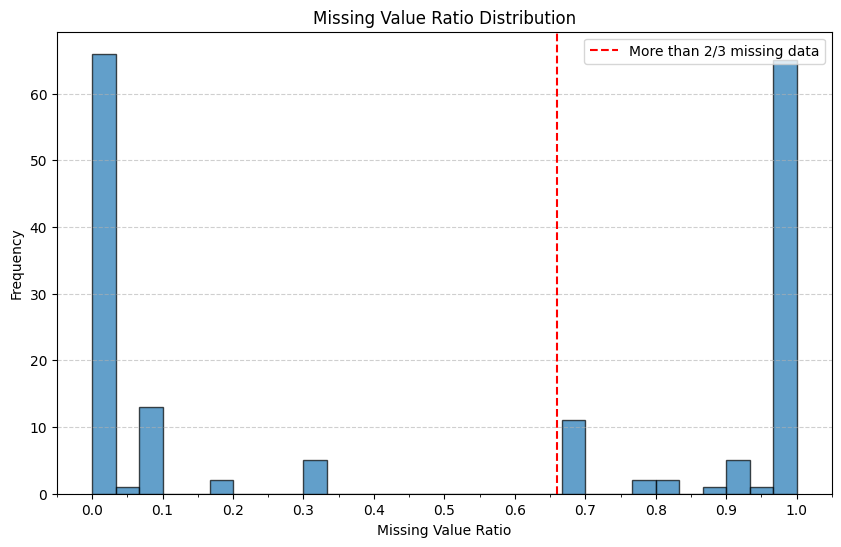
\includegraphics[width=.96\linewidth]{img/21127739/dep_missing_rate.png}
    \caption{Biểu đồ phân bố tỷ lệ thiếu giá trị của các cột}
    \label{fig:dep_missing_rate}
\end{figure}

\subsubsection{Phân tích và chuẩn hóa kiểu dữ liệu}

\paragraph{Kiểm tra kiểu dữ liệu:}
Sau khi loại bỏ các cột thiếu nhiều, kiểu dữ liệu của các cột còn lại được kiểm tra lại.

\paragraph{Chuẩn hóa cột thời gian:}
Hai cột \texttt{collectTime} (thời gian thu thập dữ liệu) và \texttt{createTime} (thời gian video được đăng tải) ban đầu có kiểu \texttt{object} và chứa giá trị dạng timestamp. Chúng đã được chuyển đổi sang kiểu \texttt{datetime} bằng hàm \texttt{pd.to\_datetime} với đơn vị là giây (\texttt{unit='s'}). Sau đó, múi giờ được chuẩn hóa về \textbf{GMT+7 (Asia/Ho\_Chi\_Minh)} để phù hợp với bối cảnh dữ liệu tại Việt Nam.

\vietnameselst
\begin{lstlisting}[language=Python]
# Convert the `collectTime` and `createTime` columns
# from POSIX to datetime64[ns] data type
video_df["collectTime"] = pd.to_datetime(video_df["collectTime"], unit="s")
video_df["createTime"] = pd.to_datetime(video_df["createTime"], unit="s")

# Change the timezone of the `collectTime` and `createTime` columns
# from UTC to Asia/Ho_Chi_Minh
video_df['createTime'] = video_df['createTime'].dt.tz_localize(
    'UTC').dt.tz_convert("Asia/Ho_Chi_Minh")
video_df['collectTime'] = video_df['collectTime'].dt.tz_localize(
    'UTC').dt.tz_convert("Asia/Ho_Chi_Minh")
\end{lstlisting}

\subsubsection{Phân tích phân bố giá trị}

\paragraph{Cột dạng số (Numerical):}
Phân tích thống kê mô tả (min, Q1, median, Q3, max) cho các cột số. Các nhận xét chính:
\begin{itemize}
    \item \texttt{authorStats.heart} và \texttt{authorStats.heartCount} có phân bố giống hệt nhau, cho thấy sự trùng lặp thông tin.
    
    \item Các cột \texttt{stats.*} và \texttt{statsV2.*} chứa thông tin tương tự (lượt xem, thích, bình luận, v.v.).
    
    \item Các cột \texttt{authorStats.friendCount} và \texttt{statsV2.repostCount} chỉ chứa một giá trị duy nhất (0.0), không mang lại nhiều thông tin biến thiên.
\end{itemize}

\paragraph{Cột không phải dạng số (Non-numerical):}
Phân tích số lượng giá trị duy nhất và tỷ lệ xuất hiện của từng giá trị. Nhận xét chính:
\begin{itemize}
    \item Nhiều cột chỉ chứa \textbf{1 giá trị duy nhất} (ví dụ: \texttt{author.commentSetting} chỉ có giá trị `0.0', \texttt{author.ftc} chỉ có `False', v.v.). Các cột này không hữu ích cho việc phân tích sự khác biệt giữa các video.
\end{itemize}

\subsubsection{Loại bỏ các cột không cần thiết/trùng lặp}

Dựa theo các phân tích trước đó, ta tiếp tục loại bỏ các cột không có nhiều ý nghĩa trong quá trình phân tích. Các cột được loại bỏ bao gồm:
\begin{itemize}
    \item \textbf{Cột ID trùng lặp}: Loại bỏ \texttt{id} và \texttt{video.videoID}, giữ lại \texttt{video.id} làm định danh chính cho video.
    
    \item \textbf{Cột thống kê cũ}: Loại bỏ các cột bắt đầu bằng \texttt{stats.*} (ví dụ: \texttt{stats.collect-\\Count}) vì trùng lặp với \texttt{statsV2.*}.
    
    \item \textbf{Cột có một giá trị duy nhất}: Loại bỏ 25 cột như \texttt{author.commentSetting}, \texttt{collected}, v.v. vì không cung cấp nhiều thông tin để phân tích.
    
    \item \textbf{Cột liên quan đến ngôn ngữ}: Loại bỏ các cột về ngôn ngữ video (ví dụ: \texttt{video.cla-\\Info.originalLanguageInfo.*}), vì dữ liệu tập trung vào khán giả Việt Nam.
    
    \item \textbf{Cột `heart' trùng lặp}: Loại bỏ \texttt{authorStats.heart} do trùng thông tin với \texttt{author-\\Stats.heartCount}.
\end{itemize}

Tổng cộng, \textbf{37 cột được loại bỏ}, giảm số lượng cột từ 87 xuống còn 50. Quá trình này được thực hiện bằng cách sử dụng các hàm phân tích của \texttt{Pandas}, như kiểm tra số giá trị duy nhất và so sánh phân phối giữa các cột.

\subsubsection{Xử lý dữ liệu thiếu trong các cột còn lại}

Đối với 50 cột còn lại, nhóm tiến hành xử lý dữ liệu thiếu như sau:
\begin{itemize}
    \item \textbf{Cột số}: Dữ liệu thiếu được điền bằng \textbf{giá trị trung vị} của cột, đảm bảo không làm lệch phân phối dữ liệu.
    \item \textbf{Cột không phải số}: Dữ liệu thiếu được điền bằng \textbf{giá trị đặc biệt} ``\texttt{others}'', tránh gây nhiễu trong phân tích.
\end{itemize}

Quá trình này đảm bảo không còn giá trị thiếu trong tập dữ liệu, với thông tin được xác nhận bằng phương thức \texttt{info()} của \texttt{Pandas}.

\subsubsection{Lưu trữ dữ liệu đã xử lý}

Kết thúc quá trình tiền xử lý, tập dữ liệu đã được làm sạch, chuẩn hóa, không còn giá trị thiếu và có kích thước \textbf{70996 hàng x 50 cột}. Kiểu dữ liệu của các cột đã phù hợp. Tập dữ liệu này được lưu dưới định dạng Parquet vào file \texttt{preprocessed\_videos.parquet} và sẵn sàng cho bước rút trích đặc trưng.

\subsection{Rút trích đặc trưng (Feature Engineering - FE)}

Sau khi làm sạch dữ liệu, nhóm tiến hành rút trích các đặc trưng quan trọng để hỗ trợ phân tích nội dung video và xây dựng công cụ viết kịch bản. Các đặc trưng bao gồm hashtag, nội dung video hàng đầu, transcript audio, thông tin món ăn, địa điểm và phân loại video.

\subsubsection{Trích xuất hashtag từ mô tả video (\texttt{desc})}

\paragraph{Quy trình:}
Từ cột \texttt{desc} chứa mô tả video, ta sử dụng biểu thức chính quy (thư viện \texttt{re} trong Python) để tìm và trích xuất các hashtag (chuỗi bắt đầu bằng ký tự \texttt{\#}). Các hashtag được chuẩn hóa bằng cách chuyển thành chữ thường và loại bỏ các dấu câu ở cuối (nếu có), đồng thời chuyển thành dạng không dấu (sử dụng thư viện \texttt{unidecode}).

\paragraph{Đặc trưng mới:}
\begin{itemize}
    \item \texttt{hashtags}: Một cột mới chứa danh sách (list) các hashtag đã được chuẩn hóa cho mỗi video.
    
    \item \texttt{hashtag\_count}: Một cột mới chứa số lượng hashtag có trong mỗi video.
\end{itemize}

\paragraph{Phân tích:}
Bảng~\ref{tab:hashtag_stats} cho thấy có đến \textbf{99,51\%} video (70.650/70.996) được đăng tải chứa ít nhất một hashtag, với trung bình \textbf{6-7 hashtag mỗi video}. Bảng~\ref{tab:popular_hashtags} cho thấy các hashtag phổ biến nhất bao gồm \texttt{ancungtiktok}, \texttt{learnontiktok}, \texttt{reviewanngon}, \texttt{xuhuong}, \texttt{mukbang}, phù hợp với chủ đề ẩm thực và xu hướng chung trên TikTok.

\begin{table}[H]
\centering
% Create two minipages side by side with vertical separator
\begin{minipage}[t]{0.47\textwidth}
    \centering
    \caption{Kết quả thống kê về hashtag}
    \label{tab:hashtag_stats}
    \renewcommand{\arraystretch}{1.3}
    \setlength{\tabcolsep}{4pt}
    \begin{tabular}{l}
    \toprule
    Total number of videos: \textbf{70996} \\
    Videos with hashtags: \textbf{70650} \\
    Percentage with hashtags: \textbf{99.51\%} \\
    Average hashtags per video: \textbf{6.85} \\
    \bottomrule
    \end{tabular}
\end{minipage}%
\hspace{0.01\textwidth}\vrule\hspace{0.01\textwidth}%
\begin{minipage}[t]{0.47\textwidth}
    \centering
    \caption{Danh sách các hashtag phổ biến}
    \label{tab:popular_hashtags}
    \renewcommand{\arraystretch}{1.3}
    \setlength{\tabcolsep}{6pt}
    \begin{tabular}{lr}
    \toprule
    \textbf{Hashtag} & \textbf{Số lần xuất hiện} \\
    \midrule
    \texttt{ancungtiktok} & 50231 \\
    \texttt{learnontiktok} & 30866 \\
    \texttt{reviewanngon} & 22232 \\
    \texttt{xuhuong} & 20930 \\
    \texttt{mukbang} & 9876 \\
    \bottomrule
    \end{tabular}
\end{minipage}
\end{table}

\subsubsection{Trích xuất đặc trưng thời gian từ \texttt{createTime}}

\paragraph{Quy trình:}
Từ cột \texttt{createTime} (đã có kiểu \texttt{datetime}), ta trích xuất thông tin về \textbf{năm} và \textbf{số thứ tự của tuần trong năm}.

\paragraph{Đặc trưng mới:}
\begin{itemize}
    \item \texttt{createTime\_year}: Năm video được đăng.
    
    \item \texttt{createTime\_week}: Số thứ tự tuần trong năm video được đăng (theo chuẩn ISO).
    
    \item \texttt{year\_week}: Một cột kết hợp năm và tuần (ví dụ: "Y2024\_W08") để dễ dàng nhóm dữ liệu theo tuần.
\end{itemize}

% Insert image
\begin{figure}[H]
    \centering
    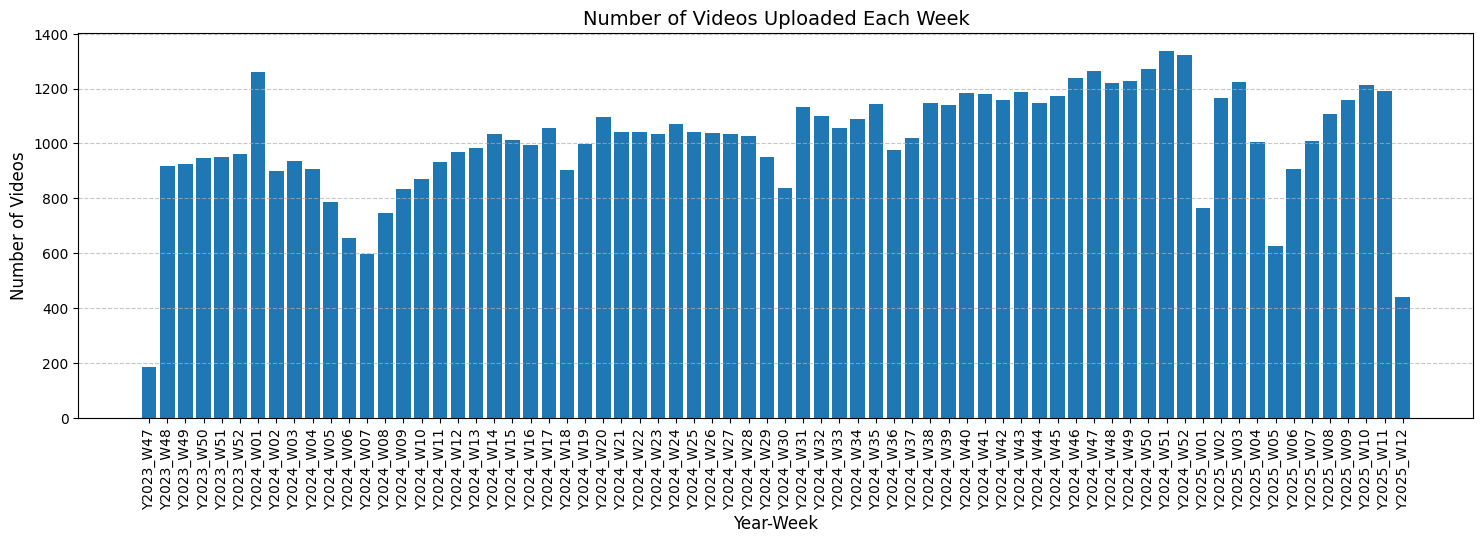
\includegraphics[width=1\linewidth]{img/21127739/num_video_per_week.png}
    \caption{Biểu đồ phân bố số lượng video được đăng tải theo các tuần trong năm}
    \label{fig:num_video_per_week}
\end{figure}

\subsubsection{Chọn top video hàng tuần để phân tích nội dung}

\paragraph{Mục tiêu:} 
Để tập trung phân tích sâu vào nội dung (transcript, món ăn, địa điểm) của các video tiềm năng nhất, nhóm quyết định chỉ xử lý một tập con các video nổi bật.

\paragraph{Tiêu chí lựa chọn:}
Nhóm đề xuất một \textbf{độ đo đánh giá} cho mỗi video dựa trên các chỉ số thống kê có sẵn trong tập dữ liệu, với \textbf{trọng tâm là số lượt xem} (\texttt{statsV2.playCount}). Cụ thể, độ đo này là \textbf{tổng có trọng số của lượt xem và các chỉ số tương tác} khác (như lượt thích, bình luận, chia sẻ) \textbf{sau khi được chuẩn hóa} để đảm bảo tính công bằng giữa các chỉ số. Mức độ đóng góp của mỗi chỉ số thống kê vào độ đo đánh giá như sau:
\begin{itemize}
    \item \texttt{statsV2.playCount} (lượt xem): 40\%.
    \item \texttt{statsV2.diggCount} (lượt thích): 25\%.
    \item \texttt{statsV2.shareCount} (lượt chia sẻ): 15\%.
    \item \texttt{statsV2.commentCount} (lượt bình luận): 10\%.
    \item Tỷ lệ tương tác: 10\%.
\end{itemize}

\paragraph{Quy trình:}
Tập dữ liệu bao gồm dữ liệu từ 70 tuần (xem Hình~\ref{fig:num_video_per_week}). Trong mỗi tuần, ta chọn ra \textbf{20\% số video có điểm số đánh giá cao nhất}. Tuy nhiên, để đảm bảo đủ dữ liệu cho phân tích, nếu 20\% số video ít hơn 100, thì ta sẽ lấy \textbf{tối thiểu 100 video} có điểm số cao nhất trong tuần đó.

\paragraph{Kết quả:}
Tạo ra một tập dữ liệu con chứa khoảng \textbf{14252 video} nổi bật nhất theo từng tuần, sẵn sàng cho các bước trích xuất nội dung tốn kém hơn về mặt tính toán (như gọi API).

\subsubsection{Trích xuất nội dung audio thành văn bản (Audio Transcription)} \label{subsubsec:transcript}

\noindent
Quy trình này được thực hiện trong file \texttt{03\_FE\_01\_01-Transcribe\_audio\_colab.ipynb} và bao gồm các bước:
\begin{enumerate}
    \item \textbf{Tái tạo URL:} Xây dựng lại URL của video TikTok từ \texttt{author.uniqueId} và \texttt{video.id} theo định dạng: \texttt{https://www.tiktok.com/@{author\_id}/video/{video\_id}}.
    
    \item \textbf{Tải audio}: Sử dụng thư viện \texttt{yt-dlp} kết hợp với \texttt{FFmpeg} để tải về \textbf{chỉ phần âm thanh} từ URL video TikTok. Audio được chuyển đổi sang định dạng WAV và lưu vào thư mục \texttt{AUDIO\_FOLDER}.
    
    \item \textbf{Chuyển đổi audio thành văn bản}: Sử dụng Gemini API (mô hình \texttt{gemini-2.0-flash}) để chuyển audio thành transcript. Dữ liệu âm thanh (file \texttt{.wav}) được đọc dưới dạng bytes và gửi kèm một \textbf{prompt} yêu cầu:
    \begin{itemize}
        \item Chuyển đổi \textbf{giọng nói tiếng Việt} trong audio thành văn bản (transcript).
        
        \item Rút ra 3 ý chính (takeaways) từ nội dung.
        
        \item Kiểm tra sự tồn tại của câu kêu gọi hành động (Call to Action - CTA).
        
        \item Kiểm tra sự tồn tại của yếu tố gây tò mò (Curiosity Gap).
        
        \item Trả về kết quả dưới dạng JSON với các trường: \texttt{transcript}, \texttt{takeaways}, \texttt{has\_call\_to-\\\_action}, \texttt{has\_curiosity\_gap}. Nếu không có giọng nói, trả về \texttt{None}.
    \end{itemize}
    
    \item \textbf{Lưu kết quả:} Kết quả JSON trả về từ API được lưu vào file \texttt{\{video\_id\}.json} trong thư mục \texttt{TRANSCRIPT\_FOLDER}. Một danh sách các \texttt{video\_id} đã xử lý được lưu lại trong file \texttt{transcribed\_video\_ids.txt} để tránh xử lý lại. 
    
    \item \textbf{Quản lý giới hạn API:} Để tránh vượt quá giới hạn lượt gọi của mỗi API, nhóm \textbf{sử dụng luân phiên} nhiều API key khác nhau. Mỗi API key được sử dụng cho \textbf{14 yêu cầu liên tiếp}, sau đó chuyển sang API key tiếp theo.
\end{enumerate}

\subsubsection{Trích xuất thông tin món ăn và địa điểm}

\noindent
Quy trình này được thực hiện trong file \texttt{03\_FE\_02\_01-Extract\_food\_location\_colab.ipynb} và dựa trên kết quả từ bước trước:
\begin{enumerate}
    \item \textbf{Dữ liệu đầu vào:} Sử dụng cột \texttt{desc} (mô tả gốc) và cột \texttt{transcript} (văn bản từ audio) của các video đã được xử lý ở Mục~\ref{subsubsec:transcript} để trích xuất thông tin về món ăn, thành phố, và quận/huyện.
    
    \item \textbf{Gọi Gemini API:} Tiếp tục sử dụng mô hình \texttt{gemini-2.0-flash}. Một \textbf{prompt} mới được thiết kế để yêu cầu mô hình phân tích nội dung \texttt{desc} và \texttt{transcript}, sau đó trích xuất:
    \begin{itemize}
        \item Danh sách các món ăn được đề cập (\texttt{foods}: list of strings).

        \item Tên thành phố (\texttt{city}: string).
        
        \item Tên quận/huyện (\texttt{district}: string).
        
        \item Prompt cũng yêu cầu mô hình trả về \texttt{None} cho các trường nếu video không thuộc chủ đề ẩm thực.
        
        \item Kết quả phải trả về đúng \textbf{định dạng JSON}.
    \end{itemize}

    \item \textbf{Lưu kết quả:} Kết quả JSON chứa thông tin món ăn và địa điểm được lưu vào file \texttt{\{video\_id\}.json} trong thư mục \texttt{new\_food\_location}. Tương tự, một danh sách các video đã xử lý được theo dõi trong file \texttt{preprocessed\_video\_ids.txt}.
    
    \item \textbf{Quản lý giới hạn API:} Nhóm cũng sử dụng nhiều API key khác nhau để \textbf{tránh vượt quá giới hạn lượt gọi}. Mỗi API key được sử dụng cho \textbf{14 yêu cầu liên tiếp}, sau đó chuyển sang API key tiếp theo.
\end{enumerate}

\subsubsection{Trích xuất đặc trưng về thể loại của video}

Và đặc trưng quan trọng cuối cùng mà ta cần rút trích là \textbf{thể loại của video}. Đây là các đặc trưng được sử dụng trực tiếp trong quá trình xây dựng công cụ hỗ trợ viết kịch bản cho video TikTok. Quy trình này sẽ được trình bày chi tiết trong Chương~\ref{sec:scriptwriting}.


% \pagebreak
% \section{CHƯƠNG 9: MỘT VÀI CÔNG CỤ BỔ TRỢ CHO VIỆC PHÁT TRIỂN KÊNH TIKTOK} \label{sec:aux_tool}

\subsection{Giới thiệu chung}

Bên cạnh công cụ cốt lõi là \textbf{công cụ hỗ trợ viết kịch bản cho video TikTok} dựa trên phân tích dữ liệu (đã trình bày ở các chương trước), nhóm nhận thấy nhu cầu của các nhà sáng tạo nội dung còn mở rộng ra các giai đoạn khác trong quá trình sản xuất video. Để đáp ứng nhu cầu này và cung cấp một bộ giải pháp toàn diện hơn, nhóm đã phát triển thêm hai công cụ bổ trợ: \textbf{công cụ hỗ trợ nghiên cứu chủ đề} và \textbf{công cụ gợi ý cách quay video ẩm thực}.

\subsection{Công cụ hỗ trợ nghiên cứu chủ đề}

% Insert image
\begin{figure}[H]
    \centering
    % Insert border box
    \frame{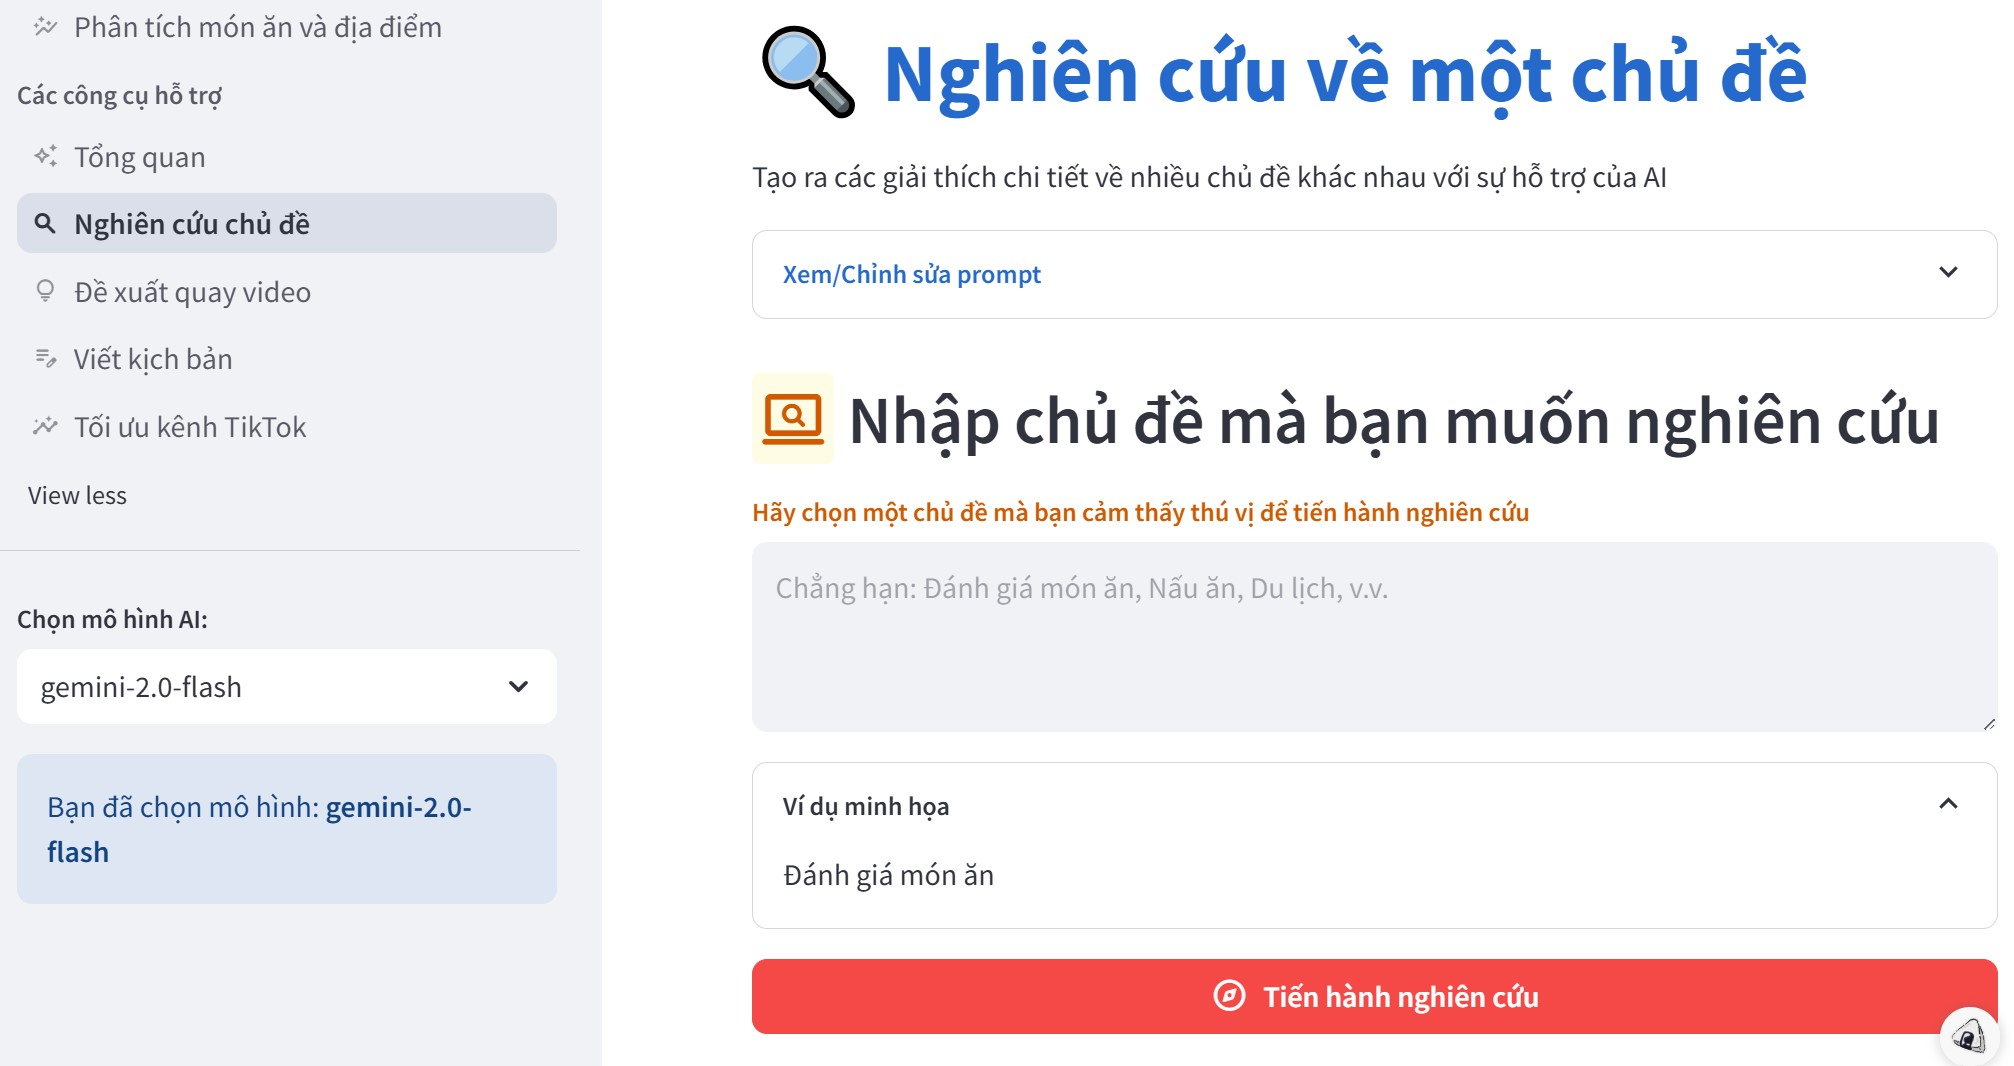
\includegraphics[width=0.99\linewidth]{img/21127739/research/research_main_page.jpg}}
    \caption{Giao diện chính của công cụ hỗ trợ nghiên cứu chủ đề}
    \label{fig:research_main_page}
\end{figure}

\subsubsection{Tổng quan}

Trong quá trình phát triển kênh TikTok, việc khám phá và thử nghiệm các chủ đề nội dung mới là yếu tố quan trọng để thu hút và giữ chân khán giả. Tuy nhiên, đối với những chủ đề mà nhà sáng tạo nội dung chưa có nhiều kinh nghiệm hoặc kiến thức nền tảng, giai đoạn nghiên cứu ban đầu có thể tốn nhiều thời gian và công sức. Để giải quyết vấn đề này, bên cạnh công cụ hỗ trợ viết kịch bản dựa trên phân tích dữ liệu TikTok, nhóm đã phát triển một công cụ bổ trợ độc lập: \textbf{Công cụ Hỗ trợ Nghiên cứu Chủ đề}.

Công cụ này được thiết kế như một \textbf{trợ lý nghiên cứu ảo}, giúp người dùng nhanh chóng tổng hợp và cấu trúc thông tin về một chủ đề bất kỳ mà họ quan tâm. Điểm khác biệt chính so với công cụ hỗ trợ viết kịch bản là công cụ này \textbf{không dựa trên việc phân tích các đặc trưng dữ liệu đã được rút trích từ video TikTok}, mà thay vào đó, nó khai thác sức mạnh của các Mô hình Ngôn ngữ Lớn (Large Language Models - LLMs) thông qua \href{https://ai.google.dev/}{Gemini API} của Google. Phần này sẽ trình bày chi tiết về mục tiêu, kiến trúc, các kỹ thuật chính được sử dụng và quy trình hoạt động của công cụ này.

\subsubsection{Mục tiêu và Lợi ích}

\noindent
Mục tiêu chính của công cụ này là cung cấp cho người dùng một phương tiện hiệu quả để:
\begin{enumerate}
    \item \textbf{Nghiên cứu nhanh chóng:} Thu thập và tổng hợp thông tin tổng quan về một chủ đề một cách nhanh chóng, thay vì phải tìm kiếm thủ công qua nhiều nguồn.
    
    \item \textbf{Hiểu biết có cấu trúc:} Thông tin trả về được trình bày một cách logic, có cấu trúc theo các khía cạnh quan trọng (tổng quan, điểm chính, ví dụ, thách thức, xu hướng, v.v.), giúp người dùng dễ dàng nắm bắt và ghi nhớ.
    
    \item \textbf{Tiết kiệm thời gian và công sức:} Giảm thiểu đáng kể thời gian dành cho việc nghiên cứu sơ bộ, cho phép người dùng tập trung nhiều hơn vào việc lên ý tưởng và sáng tạo nội dung.
    
    \item \textbf{Khám phá chủ đề mới:} Tạo điều kiện thuận lợi cho việc tìm hiểu các lĩnh vực mới mà người dùng chưa có nhiều kinh nghiệm.
\end{enumerate}

\subsubsection{Kiến trúc và Công nghệ sử dụng}

\noindent
Công cụ được xây dựng dưới dạng một ứng dụng web tương tác, sử dụng các công nghệ và kỹ thuật chính sau:
\begin{enumerate}
    \item \textbf{Framework ứng dụng web:} \textbf{Streamlit} được lựa chọn làm framework để xây dựng giao diện người dùng (UI) một cách nhanh chóng và hiệu quả. Streamlit cho phép tạo các thành phần tương tác như nút bấm, hộp chọn, vùng nhập văn bản và hiển thị kết quả động chỉ với mã Python.
    
    \item \textbf{Mô hình Ngôn ngữ Lớn (LLM):} Công cụ tận dụng khả năng \textbf{xử lý ngôn ngữ tự nhiên}, \textbf{tổng hợp thông tin} và \textbf{tạo văn bản} của các mô hình Gemini do Google cung cấp thông qua \textbf{Gemini API}. Việc sử dụng LLM cho phép công cụ nghiên cứu về hầu hết mọi chủ đề dựa trên \textit{kiến thức nền tảng rộng lớn} và \textit{khả năng truy cập thông tin} của mô hình, thay vì bị giới hạn bởi dữ liệu TikTok đã thu thập.
    
    \item \textbf{Thư viện tương tác với API:} Thư viện \texttt{google-genai} được sử dụng để gửi yêu cầu đến Gemini API và nhận kết quả trả về.
    
    \item \textbf{Kỹ thuật prompting:} Đây là kỹ thuật cốt lõi để điều khiển LLM tạo ra kết quả mong muốn. Công cụ sử dụng một cấu trúc prompt được thiết kế cẩn thận để hướng dẫn mô hình AI cung cấp thông tin theo đúng định dạng và nội dung yêu cầu.
    
    \item \textbf{Quản lý trạng thái:} \textbf{Streamlit Session State} (\texttt{st.session\_state}) được dùng để lưu trữ trạng thái của ứng dụng, chẳng hạn như prompt hiện tại do người dùng chỉnh sửa và kết quả nghiên cứu gần nhất, đảm bảo trải nghiệm người dùng liền mạch.
    
    \item \textbf{Caching:} Kỹ thuật caching (\texttt{@st.cache\_data}) được áp dụng cho các hàm đọc file (danh sách mô hình, template prompt) để tăng tốc độ tải trang và giảm thiểu việc đọc lại file không cần thiết.
\end{enumerate}

\subsubsection{Thiết kế giao diện người dùng và Luồng tương tác}

\paragraph{Giao diện người dùng:} Được thiết kế đơn giản và trực quan, bao gồm các thành phần chính:
\begin{enumerate}
    \item \textbf{Sidebar chọn mô hình:} Một menu thả xuống (\texttt{st.selectbox}) ở thanh bên (sidebar) cho phép người dùng chọn mô hình Gemini muốn sử dụng từ danh sách được đọc từ file \texttt{models/gemini\_models.txt}. Thông tin về mô hình đã chọn được hiển thị ngay bên dưới thông qua \texttt{st.info} (xem Hình~\ref{fig:research_choose_model}).
    \vspace*{-4pt}
    % Insert image
    \begin{figure}[H]
        \centering
        % Insert border box
        \frame{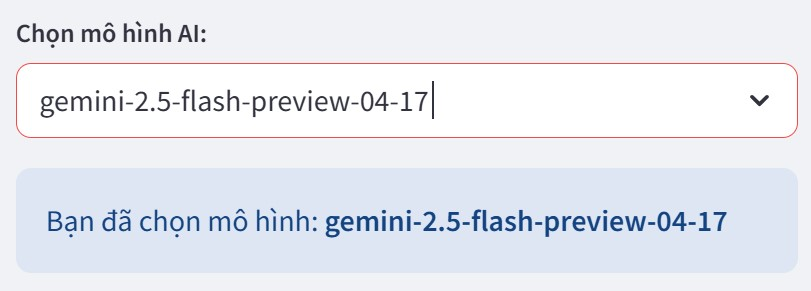
\includegraphics[width=0.55\linewidth]{img/21127739/research/research_choose_model.jpg}}
        \caption{Giao diện sidebar chọn mô hình của công cụ hỗ trợ nghiên cứu chủ đề}
        \label{fig:research_choose_model}
    \end{figure}
    \vspace*{-18pt}

    \item \textbf{Khu vực tùy chỉnh prompt:} Sử dụng \texttt{st.expander} để tạo một khu vực có thể mở rộng/thu gọn (xem Hình~\ref{fig:research_prompt_area}), chứa:
    \begin{itemize}
        \item Một vùng nhập văn bản lớn (\texttt{st.text\_area}) hiển thị prompt hiện tại (mặc định hoặc đã tùy chỉnh) và cho phép người dùng chỉnh sửa.

        \item Hai nút bấm (\texttt{st.button}) được đặt trong hai cột (\texttt{st.columns}): "\textbf{Cập nhật prompt}" để lưu thay đổi và "\textbf{Khôi phục prompt mặc định}" để quay lại nội dung gốc từ file \texttt{user\_prompt\_template.md}.
        
        \item Thông báo thành công (\texttt{st.success}) được hiển thị khi cập nhật hoặc khôi phục prompt.  
    \end{itemize}
    \vspace*{-10pt}
    % Insert image
    \begin{figure}[H]
        \centering
        % Insert border box
        \frame{
\includegraphics[width=0.8\linewidth]{img/21127739/research/research_prompt_area.jpg}}
        \caption{Giao diện khu vực tùy chỉnh prompt của công cụ hỗ trợ nghiên cứu chủ đề}
        \label{fig:research_prompt_area}
    \end{figure}
    \vspace*{-16pt}

    \item \textbf{Khu vực nhập chủ đề:} Một vùng nhập văn bản (\texttt{st.text\_area}) để người dùng nhập chủ đề cần nghiên cứu. Có một ví dụ minh họa (\texttt{st.expander}) để hướng dẫn người dùng ngay bên dưới (xem Hình~\ref{fig:research_topic_area}).
    
    \item \textbf{Nút tạo kết quả:} Nút "\textbf{Tiến hành nghiên cứu}" (\texttt{st.button} với \texttt{type="primary"}) để tiến hành gửi yêu cầu đến API (xem Hình~\ref{fig:research_topic_area}). Hệ thống sẽ kiểm tra xem người dùng đã nhập chủ đề hay chưa, nếu chưa sẽ hiển thị thông báo yêu cầu nhập chủ đề (\texttt{st.warning}).
    \vspace*{-4pt}
    % Insert image
    \begin{figure}[H]
        \centering
        % Insert border box
        \frame{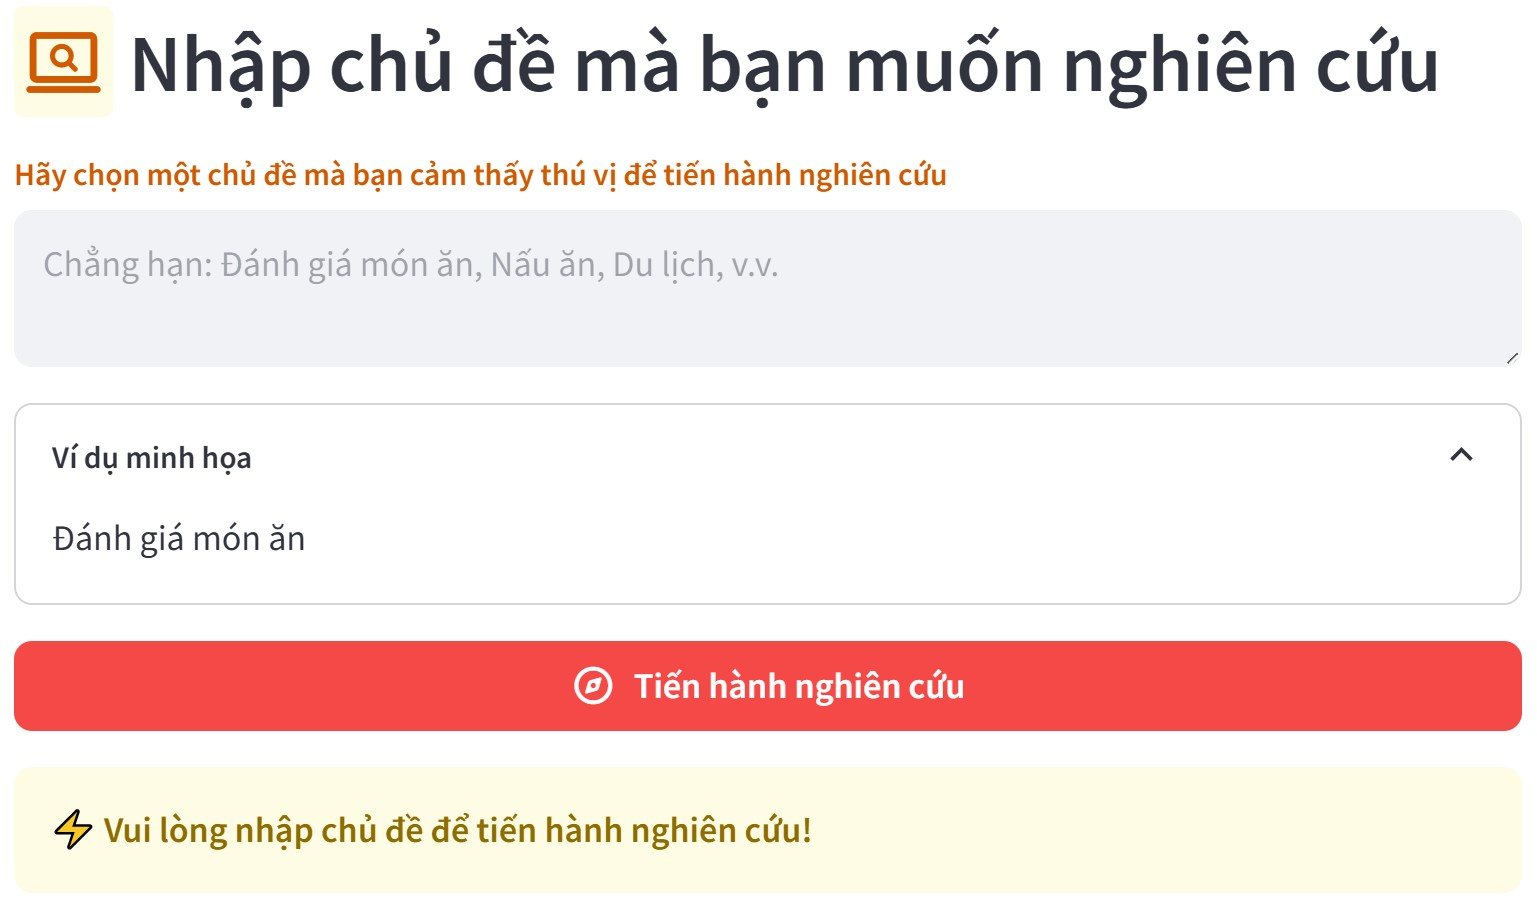
\includegraphics[width=0.8\linewidth]{img/21127739/research/research_topic_area.jpg}}
        \caption{Giao diện khu vực nhập chủ đề của công cụ hỗ trợ nghiên cứu chủ đề}
        \label{fig:research_topic_area}
    \end{figure}
    
    \item \textbf{Hiển thị kết quả:} Kết quả trả về từ API (sau khi chuẩn hóa) được hiển thị dưới dạng Markdown (\texttt{st.markdown}) trong khu vực chính (xem Hình~\ref{fig:research_result_area}). Khu vực này có thể cuộn để xem toàn bộ nội dung. Nội dung được phân chia thành các phần rõ ràng theo cấu trúc đã định nghĩa trong prompt, giúp người dùng dễ dàng theo dõi và hiểu thông tin.
    % Insert image
    \begin{figure}[H]
        \centering
        % Insert border box
        \frame{
\includegraphics[width=0.67\linewidth]{img/21127739/research/research_result_area.jpg}}
        \caption{Giao diện khu vực hiển thị kết quả của công cụ hỗ trợ nghiên cứu chủ đề}
        \label{fig:research_result_area}
    \end{figure}
    \vspace*{-14pt}

    \item \textbf{Lưu kết quả:} Hai nút bấm (\texttt{st.button} và \texttt{st.download\_button}) được đặt trong hai cột (\texttt{st.columns}) dưới phần kết quả (xem Hình~\ref{fig:research_save_result}), cho phép người dùng:
    \begin{itemize}
        \item Sao chép kết quả vào clipboard (sử dụng thư viện \texttt{pyperclip}).

        \item Tải kết quả xuống dưới dạng file Markdown (\texttt{.md}).        
    \end{itemize}
    \vspace*{-4pt}
    % Insert image
    \begin{figure}[H]
        \centering
        % Insert border box
        \frame{
\includegraphics[width=0.67\linewidth]{img/21127739/research/research_save_result.jpg}}
        \caption{Giao diện khu vực lưu kết quả của công cụ hỗ trợ nghiên cứu chủ đề}
        \label{fig:research_save_result}
    \end{figure}
\end{enumerate}

\paragraph{Luồng tương tác của người dùng:} Người dùng sẽ thực hiện các bước sau để sử dụng công cụ:
\begin{enumerate}
    \item (Tùy chọn) Chọn mô hình AI từ sidebar.

    \item (Tùy chọn) Mở rộng khu vực prompt, xem và chỉnh sửa nếu cần, sau đó nhấn "Cập nhật prompt" hoặc "Khôi phục prompt mặc định".
    
    \item Nhập chủ đề muốn nghiên cứu vào ô văn bản.
    
    \item Nhấn nút "Tiến hành nghiên cứu".
    
    \item Chờ đợi trong khi hệ thống hiển thị trạng thái "Đang nghiên cứu..." (\texttt{st.spinner}).
    
    \item Xem kết quả được hiển thị.
    
    \item (Tùy chọn) Sao chép hoặc tải xuống kết quả.
\end{enumerate}

\subsubsection{Kỹ thuật Prompting}

Hiệu quả của công cụ phụ thuộc rất lớn vào cách thiết kế prompt để giao tiếp với mô hình Gemini. Nhóm đã áp dụng phương pháp sử dụng kết hợp \textbf{System Prompt} và \textbf{User Prompt} để tối ưu hóa khả năng tạo nội dung của mô hình:
\begin{enumerate}
    \item \textbf{System Prompt (\texttt{system\_prompt\_template.md}):}
    \begin{itemize}
        \item \textbf{Mục đích:} Định nghĩa vai trò và hướng dẫn tổng quát cho mô hình AI. Prompt này yêu cầu mô hình đóng vai là ``\textit{chuyên gia nghiên cứu với kiến thức sâu rộng}''.

        \item \textbf{Định dạng đầu ra:} Quan trọng nhất, system prompt yêu cầu mô hình trả lời theo định dạng Markdown với một cấu trúc gồm 7 phần rõ ràng: \texttt{Overview}, \texttt{Key Points}, \texttt{Examples}, \texttt{Challenges}, \texttt{Best Practices}, \texttt{Trends}, và \texttt{Resources}. Nó cũng nhấn mạnh các yêu cầu về tính rõ ràng, súc tích, chính xác và việc chỉ trả về nội dung bên trong khối Markdown.
        
        \item \textbf{Kỹ thuật:} Sử dụng kỹ thuật "\textbf{Role Playing}" (đóng vai) và "\textbf{Output Formatting}" (định dạng đầu ra) để kiểm soát hành vi và cấu trúc kết quả của LLM.
    \end{itemize}

    \item \textbf{User Prompt (\texttt{user\_prompt\_template.md} và tùy chỉnh của người dùng):}
    \begin{itemize}
        \item \textbf{Mục đích:} Cung cấp yêu cầu cụ thể hơn về nội dung cho từng phần trong cấu trúc đã định nghĩa ở system prompt. Prompt mặc định liệt kê lại các phần mong muốn và mô tả ngắn gọn nội dung của từng phần.

        \item \textbf{Tính linh hoạt:} Người dùng có thể tùy chỉnh user prompt này thông qua giao diện (\texttt{st.text\_area}). Ví dụ, họ có thể yêu cầu tập trung sâu hơn vào phần "Challenges" hoặc bổ sung một phần mới như "Target Audience".
        
        \item \textbf{Kết hợp:} Khi gửi yêu cầu đến API, system prompt được gửi trước, theo sau là một câu dẫn (``\textit{Hãy giúp tôi tạo ra một bài giải thích chi tiết về chủ đề [topic].}'') và cuối cùng là nội dung user prompt (mặc định hoặc đã tùy chỉnh).
    \end{itemize}

    \item \textbf{Khôi phục Prompt:} Chức năng khôi phục về prompt mặc định (\texttt{default\_user\_prompt}) đảm bảo người dùng luôn có thể quay lại trạng thái ban đầu nếu việc tùy chỉnh không như ý.
\end{enumerate}

Kỹ thuật prompting này giúp đảm bảo tính nhất quán trong cấu trúc đầu ra, đồng thời mang lại sự linh hoạt cho người dùng để điều chỉnh nội dung theo nhu cầu nghiên cứu cụ thể.

\subsubsection{Tương tác với Gemini API và Xử lý kết quả}
\begin{enumerate}
    \item \textbf{Lựa chọn mô hình:} Như đã đề cập, người dùng có thể chọn các mô hình Gemini khác nhau. Hàm \texttt{read\_available\_gemini\_models} đọc danh sách các mô hình có sẵn từ file \texttt{models/gemini\_models.txt} và hiển thị trong \texttt{st.selectbox}. Việc chọn mô hình nhanh hơn (\texttt{gemini-2.0-flash}, \texttt{gemini-2.5-flash}) sẽ cho kết quả nhanh hơn nhưng có thể kém chi tiết hơn so với mô hình mạnh hơn (\texttt{gemini-2.5-pro}).
    
    \item \textbf{Gửi yêu cầu:} Khi người dùng nhấn nút "Tiến hành nghiên cứu", hàm \texttt{generate\_content} (trong file \texttt{research.py}, gọi đến \texttt{client.models.generate\_content} của thư viện \texttt{google-\\genai}) được thực thi. Hàm này nhận vào system prompt, user prompt (đã được định dạng cùng với chủ đề) và tên mô hình đã chọn. API key được sử dụng để xác thực yêu cầu. (\textit{Quá trình này thường mất khoảng 15 giây.})
    
    \item \textbf{Nhận và Chuẩn hóa phản hồi:} Gemini API trả về một đối tượng response. Phần nội dung văn bản (\texttt{response.text}) thường được bao bọc trong khối mã Markdown (nội dung chính được bao bọc bởi các ký tự đánh dấu). Hàm \texttt{standardize\_response} được sử dụng để loại bỏ các ký tự đánh dấu không cần thiết, chỉ giữ lại nội dung Markdown thuần túy.
    
    \item \textbf{Hiển thị và Lưu trữ:} Kết quả Markdown đã chuẩn hóa được hiển thị trực tiếp trên giao diện bằng \texttt{st.markdown}. Đồng thời, kết quả này được lưu vào \texttt{st.session\_state.last\_re-\\search\_response} để có thể sử dụng cho chức năng sao chép và tải xuống.
    
    \item \textbf{Sao chép và Tải xuống:}
    \begin{itemize}
        \item Nút "Sao chép nội dung" sử dụng thư viện \texttt{pyperclip} (\texttt{pyperclip.copy()}) để đưa nội dung trong \texttt{st.session\_state.last\_research\_response} vào clipboard hệ thống (\textit{tiện lợi cho việc dán vào tài liệu hoặc ứng dụng khác}).
        
        \item Nút "Tải xuống nội dung" sử dụng \texttt{st.download\_button}, truyền vào nội dung (có thể thêm tiêu đề ``\texttt{\# Chủ đề: [topic]}'') và định dạng file là \texttt{research\_topic.md} với kiểu MIME là \texttt{text/plain} (\textit{phù hợp cho chỉnh sửa hoặc lưu trữ lâu dài}).
    \end{itemize}
    
\end{enumerate}

\subsubsection{Minh họa cách sử dụng công cụ}

% Providing a practical example
Để minh họa cách công cụ hoạt động, nhóm đã quay video hướng dẫn sử dụng công cụ này, người dùng có thể tham khảo video demo tại \href{https://youtu.be/m-cdmfVc2rk?list=PL3SfxVDJ_Zc6DvBKVd6xUc-exmt0AyA7x&t=246}{đây} (\textit{từ phút 4:10 đến 8:32}). Trong ví dụ minh họa, người dùng muốn nghiên cứu về chủ đề "Đánh giá món ăn" (Food Review) để tạo video TikTok. Ví dụ này cho thấy công cụ giúp người dùng nhanh chóng thu thập thông tin có cấu trúc, hỗ trợ quá trình sáng tạo nội dung.

\subsection{Công cụ gợi ý cách quay video ẩm thực}

% Insert image
\begin{figure}[H]
    \centering
    % Insert border box
    \frame{
\includegraphics[width=0.99\linewidth]{img/21127739/suggestion/suggestion_main_page.jpg}}
    \caption{Giao diện chính của công cụ gợi ý cách quay video ẩm thực}
    \label{fig:suggestion_main_page}
\end{figure}

\subsubsection{Tổng quan}

Trong quy trình sáng tạo nội dung trên TikTok, sau giai đoạn lên ý tưởng và viết kịch bản, việc thực hiện các cảnh quay (filming) đóng vai trò then chốt, quyết định phần lớn chất lượng hình ảnh và cảm xúc của video thành phẩm. Đối với lĩnh vực ẩm thực, việc quay phim đòi hỏi sự chú ý đặc biệt đến các yếu tố như góc máy làm nổi bật món ăn, ánh sáng hấp dẫn, âm thanh sống động và cách thể hiện tương tác tự nhiên. Tuy nhiên, không phải nhà sáng tạo nội dung nào cũng có đủ kinh nghiệm hoặc kiến thức chuyên sâu về kỹ thuật quay phim cho từng thể loại video ẩm thực cụ thể.

Để giải quyết thách thức này và bổ sung vào bộ công cụ hỗ trợ phát triển kênh TikTok, nhóm đã xây dựng \textbf{Công cụ Gợi ý Cách quay Video Ẩm thực}. Công cụ này hoạt động như một \textbf{cố vấn sản xuất ảo}, cung cấp những lời khuyên và gợi ý kỹ thuật quay phim chi tiết, được cá nhân hóa dựa trên ý tưởng video và thể loại ẩm thực mà người dùng lựa chọn. Tương tự công cụ nghiên cứu chủ đề, công cụ này cũng khai thác sức mạnh của Mô hình Ngôn ngữ Lớn (LLM) tiên tiến thông qua \href{https://ai.google.dev/}{Gemini API}, tập trung vào kỹ thuật prompting để tạo ra các gợi ý chuyên sâu. Phần này sẽ đi sâu vào phân tích mục tiêu, kiến trúc, các kỹ thuật chính và quy trình hoạt động của công cụ gợi ý quay video.

\subsubsection{Mục tiêu và Lợi ích}

\noindent
Công cụ được xây dựng với các mục tiêu cụ thể sau:
\begin{enumerate}
    \item \textbf{Nâng cao chất lượng hình ảnh:} Cung cấp các gợi ý về góc quay, ánh sáng, bố cục để giúp video trông chuyên nghiệp và hấp dẫn hơn về mặt thị giác.

    \item \textbf{Tối ưu hóa kỹ thuật quay:} Đề xuất các kỹ thuật quay phù hợp (slow-motion, cận cảnh, góc nhìn thứ nhất, v.v.) cho từng thể loại và nội dung cụ thể.
    
    \item \textbf{Cải thiện âm thanh:} Gợi ý cách thu âm, xử lý tạp âm và lựa chọn nhạc nền phù hợp để tăng trải nghiệm nghe của khán giả.
    
    \item \textbf{Tăng tính hấp dẫn của nội dung:} Đưa ra lời khuyên về cách tương tác, kể chuyện và trình bày món ăn một cách lôi cuốn.
    
    \item \textbf{Hỗ trợ theo thể loại:} Cung cấp gợi ý chuyên biệt cho các thể loại video ẩm thực phổ biến (review, nấu ăn, mukbang).
    
    \item \textbf{Tiết kiệm thời gian chuẩn bị:} Giúp người dùng, đặc biệt là những người mới, có sự chuẩn bị tốt hơn cho buổi quay, giảm thiểu thời gian thử nghiệm và sai sót.
\end{enumerate}

\subsubsection{Kiến trúc và Công nghệ sử dụng}

\noindent
Công cụ gợi ý quay video được triển khai dưới dạng ứng dụng web, sử dụng các thành phần công nghệ tương tự như công cụ nghiên cứu chủ đề:
\begin{enumerate}
    \item \textbf{Framework ứng dụng web:} \textbf{Streamlit} tiếp tục được sử dụng để xây dựng giao diện người dùng thân thiện và các thành phần tương tác (tham khảo file \texttt{suggestion.py}).

    \item \textbf{Mô hình Ngôn ngữ Lớn (LLM):} Công cụ dựa vào khả năng hiểu ngữ cảnh, kiến thức chuyên môn (được mô phỏng qua prompt) và khả năng tạo văn bản của các mô hình \textbf{Gemini API} để đưa ra các gợi ý quay phim.
    
    \item \textbf{Thư viện tương tác với API:} Thư viện \texttt{google-genai} được dùng để giao tiếp với Gemini API.
    
    \item \textbf{Kỹ thuật Prompting theo ngữ cảnh:} Điểm nhấn kỹ thuật của công cụ này là việc sử dụng các \textbf{prompt chuyên biệt} cho từng thể loại video ẩm thực, kết hợp với mô tả ý tưởng của người dùng để tạo ra gợi ý phù hợp nhất.
    
    \item \textbf{Quản lý trạng thái:} \textbf{Streamlit Session State} (\texttt{st.session\_state}) được dùng để lưu trữ gợi ý gần nhất được tạo ra, cho phép người dùng xem lại và thực hiện các thao tác lưu trữ.
    
    \item \textbf{Caching:} Kỹ thuật caching (\texttt{@st.cache\_data}) được áp dụng cho việc đọc danh sách mô hình và nội dung các file prompt template, tối ưu hóa hiệu năng ứng dụng.
\end{enumerate}

\subsubsection{Thiết kế giao diện người dùng và Luồng tương tác}

\paragraph{Giao diện người dùng:} Giao diện người dùng được thiết kế để người dùng dễ dàng nhập thông tin và nhận gợi ý:
\begin{enumerate}
    \item \textbf{Chọn loại video và mô hình AI:} (Xem Hình~\ref{fig:suggestion_choose_video_type_and_model})
    \begin{itemize}
        \item Sử dụng hai cột (\texttt{st.columns}) để bố trí các lựa chọn.

        \item \textbf{Chọn loại video:} Người dùng chọn một trong ba loại video ẩm thực (\textit{Video review món ăn hoặc quán ăn}, \textit{Video mukbang}, \textit{Video hướng dẫn nấu ăn}) thông qua nút \texttt{st.radio}. Danh sách các loại video được định nghĩa trong biến \texttt{VIDEO\_TYPES}.
        
        \item \textbf{Chọn mô hình AI:} Người dùng chọn mô hình Gemini mong muốn từ danh sách (đọc từ file \texttt{models/gemini\_models.txt}) bằng \texttt{st.selectbox}.
        
        \item Thông tin về lựa chọn của người dùng được hiển thị xác nhận bằng \texttt{st.info}.
    \end{itemize}
    % Insert image
    \begin{figure}[H]
        \centering
        % Insert border box
        \frame{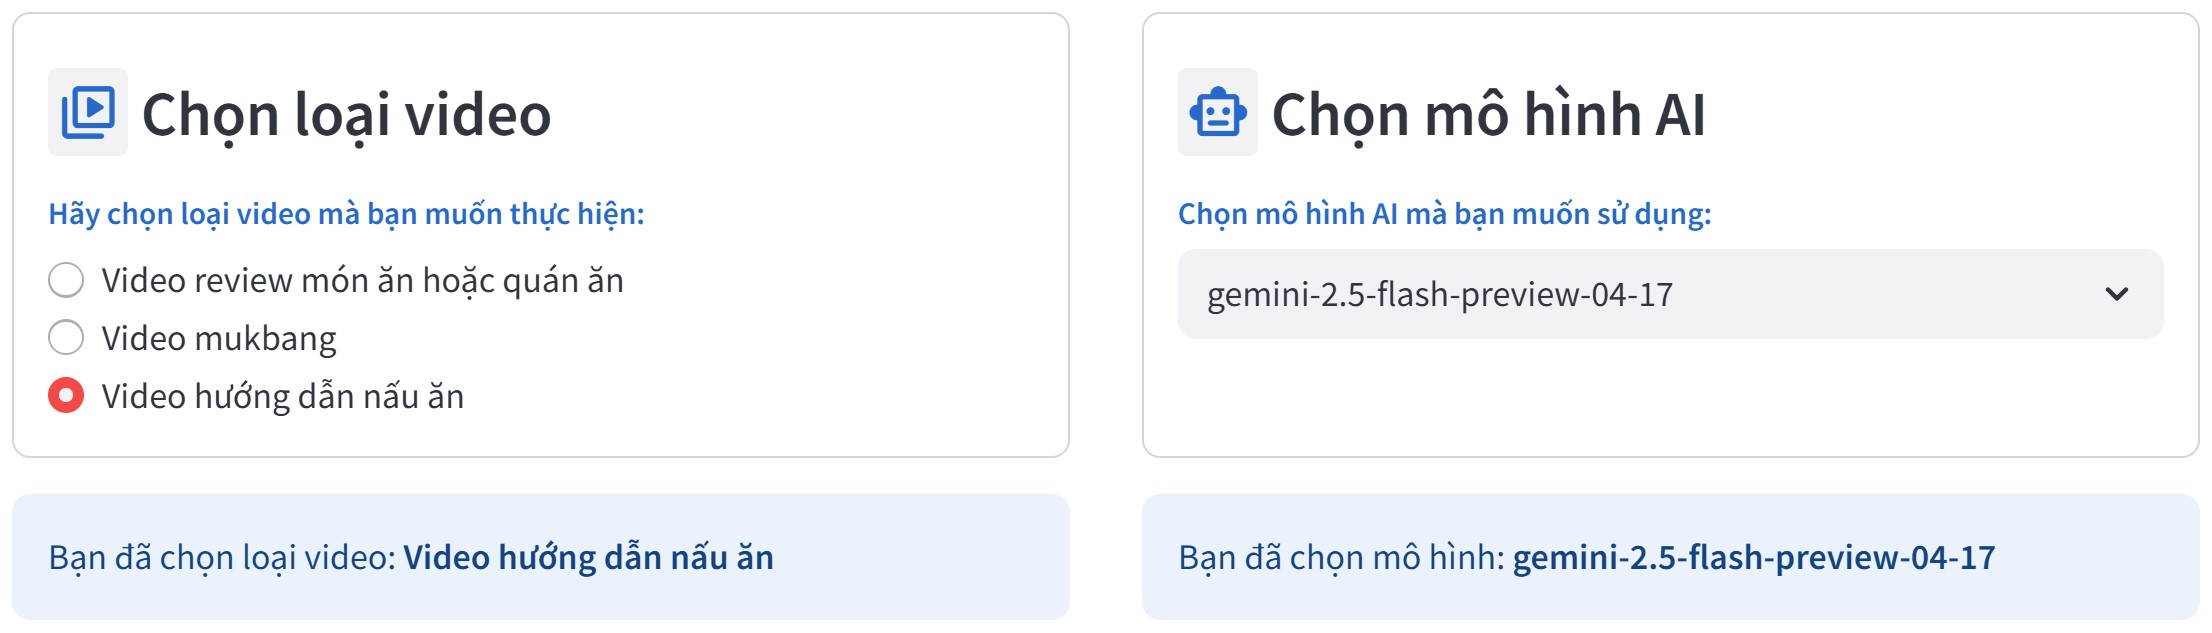
\includegraphics[width=0.9\linewidth]{img/21127739/suggestion/suggestion_choose_video_type_and_model.jpg}}
        \caption{Giao diện chọn loại video và mô hình AI của công cụ gợi ý cách quay video ẩm thực}
        \label{fig:suggestion_choose_video_type_and_model}
    \end{figure}

    \item \textbf{Nhập mô tả video:} (Xem Hình~\ref{fig:suggestion_input_description})
    \begin{itemize}
        \item Một vùng nhập văn bản lớn (\texttt{st.text\_area}) cho phép người dùng mô tả chi tiết ý tưởng video của họ (món ăn, địa điểm, phong cách, mục tiêu, v.v.).

        \item Có một ví dụ minh họa (\texttt{st.expander}) để người dùng tham khảo cách mô tả hiệu quả.
    \end{itemize}
    \item \textbf{Nút tạo gợi ý:} Nút "Tạo gợi ý" (\texttt{st.button} với \texttt{type="primary"}) để bắt đầu quá trình tạo gợi ý. Hệ thống sẽ kiểm tra xem người dùng đã nhập mô tả hay chưa, nếu chưa sẽ hiển thị thông báo yêu cầu nhập mô tả thông qua \texttt{st.warning} (xem Hình~\ref{fig:suggestion_input_description}).
    % Insert image
    \begin{figure}[H]
        \centering
        % Insert border box
        \frame{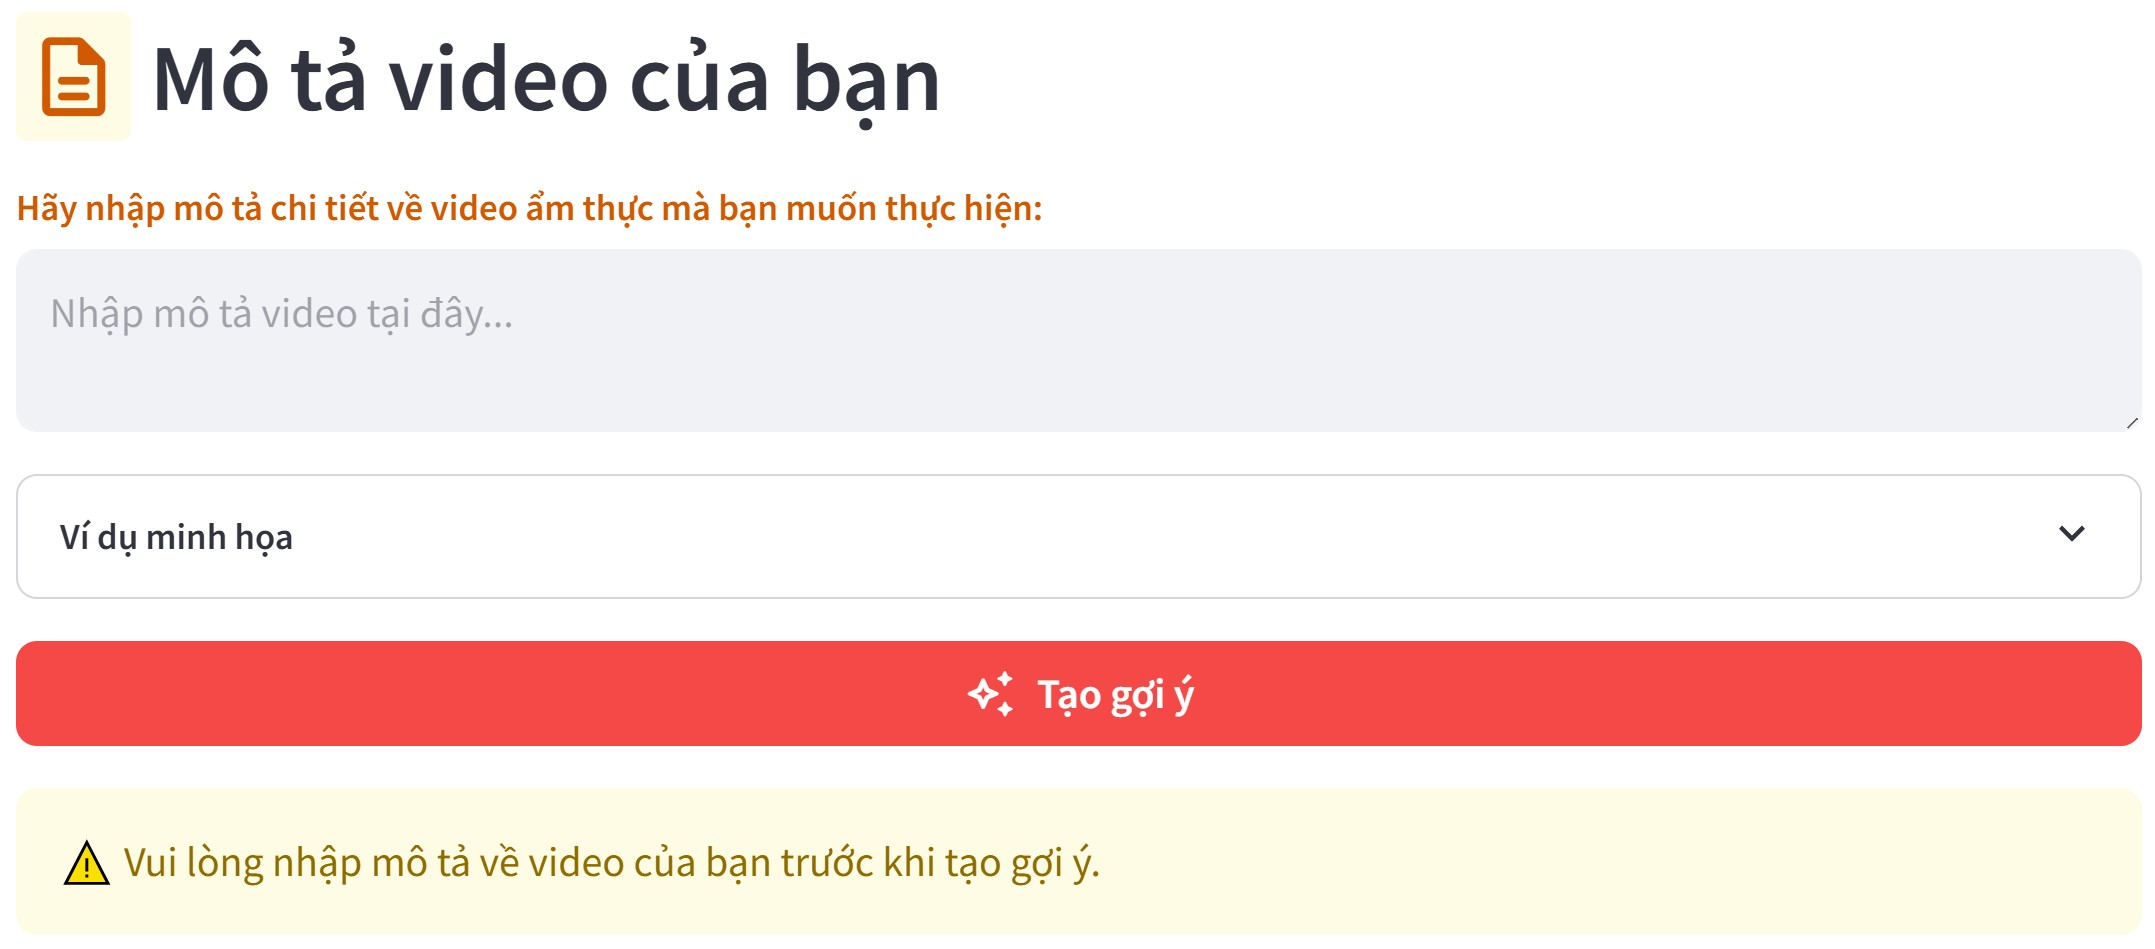
\includegraphics[width=0.9\linewidth]{img/21127739/suggestion/suggestion_input_description.jpg}}
        \caption{Giao diện nhập mô tả video của công cụ gợi ý cách quay video ẩm thực}
        \label{fig:suggestion_input_description}
    \end{figure}

    \item \textbf{Hiển thị gợi ý:} (Xem Hình~\ref{fig:suggestion_result})
    \begin{itemize}
        \item Trong khi chờ đợi, \texttt{st.spinner} hiển thị thông báo "Đang tạo gợi ý...".

        \item Kết quả gợi ý (dạng Markdown) trả về từ API được lưu vào \texttt{st.session\_state.sug-\\gestion} và hiển thị trên giao diện bằng \texttt{st.markdown}.
    \end{itemize}
    % Insert image
    \begin{figure}[H]
        \centering
        % Insert border box
        \frame{
\includegraphics[width=0.9\linewidth]{img/21127739/suggestion/suggestion_result.jpg}}
        \caption{Giao diện hiển thị gợi ý của công cụ gợi ý cách quay video ẩm thực}
        \label{fig:suggestion_result}
    \end{figure}

    \item \textbf{Lưu kết quả:} (Xem Hình~\ref{fig:suggestion_save_result}) Tương tự công cụ nghiên cứu, hai nút bấm trong hai cột (\texttt{st.columns}) cho phép:
    \begin{itemize}
        \item Sao chép gợi ý vào clipboard (\texttt{pyperclip.copy()}).
        
        \item Tải gợi ý xuống dưới dạng file Markdown (\texttt{.md}) bằng \texttt{st.download\_button}.
    \end{itemize}
    % Insert image
    \begin{figure}[H]
        \centering
        % Insert border box
        \frame{
\includegraphics[width=0.9\linewidth]{img/21127739/suggestion/suggestion_save_result.jpg}}
        \caption{Giao diện lưu kết quả của công cụ gợi ý cách quay video ẩm thực}
        \label{fig:suggestion_save_result}
    \end{figure}

\end{enumerate}

\paragraph{Luồng tương tác của người dùng:} Người dùng sẽ thực hiện các bước sau để sử dụng công cụ:
\begin{enumerate}
    \item Chọn loại video ẩm thực muốn thực hiện.

    \item (Tùy chọn) Chọn mô hình AI muốn sử dụng.
    
    \item Nhập mô tả chi tiết về ý tưởng video.
    
    \item Nhấn nút "Tạo gợi ý".
    
    \item Xem các gợi ý chi tiết được hiển thị.
    
    \item (Tùy chọn) Sao chép hoặc tải xuống các gợi ý.
\end{enumerate}

\subsubsection{Kỹ thuật Prompting chuyên biệt theo thể loại video}

Đây là yếu tố kỹ thuật cốt lõi giúp công cụ đưa ra những gợi ý phù hợp và chuyên sâu. Thay vì dùng một prompt chung, công cụ sử dụng các prompt riêng biệt được thiết kế cho từng thể loại video ẩm thực:
\begin{enumerate}
    \item \textbf{Cấu trúc Prompt:} Mỗi prompt template (lưu trong các file \texttt{.md} tương ứng: \texttt{food\_review-\\\_template.md}, \texttt{cooking\_template.md}, \texttt{mukbang\_template.md}) đều có cấu trúc chung:
    \begin{itemize}
        \item \textbf{Định nghĩa vai trò (Role Playing):} Yêu cầu LLM đóng vai là "chuyên gia sản xuất video chuyên nghiệp" với kinh nghiệm trong thể loại video tương ứng (review, nấu ăn, hoặc mukbang).

        \item \textbf{Xác định đầu vào:} Nêu rõ rằng người dùng sẽ cung cấp thông tin/mô tả về video họ muốn làm.
        
        \item \textbf{Yêu cầu đầu ra:} Liệt kê chi tiết các hạng mục cần gợi ý, được trình bày dưới dạng danh sách gạch đầu dòng với các tiêu đề in đậm (định dạng Markdown). Các hạng mục này bao gồm những khía cạnh quan trọng nhất của việc quay phim ẩm thực:
        \begin{itemize}
            \item \textit{Setup máy quay \& Góc quay}

            \item \textit{Ánh sáng \& Âm thanh}
            
            \item \textit{Giải thích \& Hướng dẫn chi tiết} (cho video nấu ăn) hoặc \textit{Chi tiết về phỏng vấn \& giao tiếp} (cho video review) hoặc \textit{Nêu cảm nhận \& Tương tác với khán giả} (cho video mukbang)
            
            \item \textit{Hiệu ứng \& Chuyển cảnh}
            
            \item \textit{Storytelling \& CTA}
            
            \item \textit{SEO \& Thương hiệu} (cho video review)
        \end{itemize}

        \item \textbf{Yêu cầu định dạng:} Yêu cầu trả lời bằng định dạng Markdown.
    \end{itemize}

    \item \textbf{Nội dung chuyên biệt:} Mặc dù có cấu trúc chung, nội dung yêu cầu chi tiết trong từng hạng mục của mỗi prompt được điều chỉnh để phù hợp với đặc thù của thể loại đó:
    \begin{itemize}
        \item \textbf{Review:} Nhấn mạnh vào góc quay đa dạng (toàn cảnh quán, cận cảnh món ăn), cách phỏng vấn chủ quán, xây dựng câu chuyện, tạo không khí đặc trưng của quán.
        
        \item \textbf{Nấu ăn:} Tập trung vào góc quay chi tiết các bước chế biến, ánh sáng làm nổi bật món ăn, giải thích rõ ràng, tạo không khí ấm cúng trong bếp.
        
        \item \textbf{Mukbang:} Chú trọng góc quay thể hiện cảm xúc khi ăn, âm thanh ASMR (nếu có), cách tương tác tự nhiên, tạo không khí vui vẻ, thân mật.
    \end{itemize}
    
    \item \textbf{Kết hợp prompt và mô tả từ người dùng:} Khi người dùng chọn loại video và nhập mô tả, hàm \texttt{generate\_suggestion} (trong file \texttt{suggestion.py}) sẽ:
    \begin{itemize}
        \item Xác định file prompt template tương ứng dựa trên \texttt{video\_type} (thông qua dictionary \texttt{VIDEO\_TYPE\_TO\_PROMPT}).
        
        \item Đọc nội dung prompt từ file đó bằng hàm \texttt{read\_prompt\_file} (có sử dụng decorator \texttt{@st.cache\_data}).
        
        \item Gửi nội dung prompt này (đóng vai trò system prompt/hướng dẫn) cùng với \texttt{user\_des-\\cription} (mô tả của người dùng) đến Gemini API.
    \end{itemize}
\end{enumerate}

Cách tiếp cận này cho phép LLM hiểu rõ ngữ cảnh (thể loại video) và yêu cầu cụ thể (mô tả của người dùng), từ đó đưa ra những gợi ý quay phim mang tính chuyên môn và sát với thực tế hơn.

\subsubsection{Tương tác với Gemini API và Xử lý kết quả}

\noindent
Quy trình tương tác với API và xử lý kết quả tương tự như công cụ nghiên cứu chủ đề:
\begin{enumerate}
    \item \textbf{Lựa chọn mô hình AI:} Người dùng chọn mô hình AI qua \texttt{st.selectbox}, mỗi mô hình có đặc điểm riêng về độ chi tiết và tốc độ phản hồi. Một số mô hình tiêu biểu bao gồm:
    \begin{itemize}
        \item \textbf{Gemini-2.5-pro}: Mô hình thử nghiệm tiên tiến nhất, được Google công bố vào tháng 3 năm 2025, cung cấp câu trả lời chi tiết nhưng có thể chậm hơn do tính chất thử nghiệm.
        
        \item \textbf{Gemini-2.0-flash}: Mô hình ổn định, được Google khuyến nghị cho các nhà phát triển, nổi bật với tốc độ phản hồi nhanh và chất lượng tốt trên nhiều tác vụ.
        
        \item \textbf{Gemini-2.5-flash}: Mô hình thử nghiệm mới, ra mắt vào giữa tháng 4 năm 2025, cân bằng giữa tốc độ của \textbf{Gemini-2.0-flash} và độ chi tiết của \textbf{Gemini-2.5-pro}.
    \end{itemize}

    \item \textbf{Gửi yêu cầu:} Hàm \texttt{generate\_suggestion} gọi \texttt{client.models.generate\_content} với prompt template phù hợp, mô tả của người dùng và tên mô hình đã chọn.
    
    \item \textbf{Nhận và Hiển thị phản hồi:} Kết quả dạng text được trả về và hiển thị bằng \texttt{st.markdown}.
    
    \item \textbf{Lưu trữ và Tương tác:} Kết quả được lưu vào \texttt{st.session\_state} để hỗ trợ sao chép (\texttt{pyperclip.copy}) và tải xuống (\texttt{st.download\_button} với tên file \texttt{video\_suggestion.md}).
\end{enumerate}

\subsubsection{Minh họa cách sử dụng công cụ}

% Providing a practical example
Để minh họa cách công cụ hoạt động, nhóm đã quay video hướng dẫn sử dụng công cụ này, người dùng có thể tham khảo video demo tại \href{https://youtu.be/m-cdmfVc2rk?list=PL3SfxVDJ_Zc6DvBKVd6xUc-exmt0AyA7x&t=512}{đây} (\textit{từ phút 8:32 đến 11:04}). Trong ví dụ minh họa, người dùng muốn quay video review một quán ăn vặt dành cho học sinh sinh viên. Công cụ gợi ý cách quay video sẽ giúp người dùng có được những gợi ý chi tiết về cách quay, ánh sáng, âm thanh và cách tương tác với chủ quán để tạo ra một video hấp dẫn và chất lượng.


% \pagebreak
% \section{CHƯƠNG 10: BÀN LUẬN VÀ KẾT LUẬN}

\subsection{Bàn luận}

Đồ án ``\textbf{Phân tích dữ liệu TikTok và Xây dựng công cụ hỗ trợ viết kịch bản dành cho các video TikTok}'' đã được thực hiện với mục tiêu ứng dụng khoa học dữ liệu và trí tuệ nhân tạo để hỗ trợ các nhà sáng tạo nội dung, đặc biệt trong lĩnh vực ẩm thực. Qua quá trình thực hiện, nhóm đã đạt được những kết quả đáng kể và rút ra nhiều bài học kinh nghiệm giá trị.

\subsubsection{Tóm tắt các kết quả đạt được}

\begin{enumerate}
    \item \textbf{Hoàn thiện Quy trình Khoa học Dữ liệu:} Nhóm đã thực hiện thành công một quy trình khoa học dữ liệu bài bản, bao gồm các giai đoạn: thu thập dữ liệu từ TikTok, tiền xử lý và làm sạch dữ liệu, rút trích các đặc trưng quan trọng (như hashtag, thông tin thời gian, nội dung audio, món ăn, địa điểm), phân tích khám phá dữ liệu thông qua dashboard trực quan, và cuối cùng là xây dựng các công cụ hỗ trợ. Quá trình này không chỉ tạo ra một tập dữ liệu có chất lượng về video ẩm thực trên TikTok mà còn giúp nhóm hiểu sâu hơn về đặc điểm và xu hướng của loại nội dung này.
    
    \item \textbf{Xây dựng Công cụ Hỗ trợ Viết Kịch bản:} Công cụ cốt lõi của đồ án đã được phát triển thành công, có khả năng tự động tạo ra gợi ý kịch bản chi tiết cho video ẩm thực dựa trên các đặc trưng dữ liệu đã phân tích và mô tả ý tưởng do người dùng cung cấp. Công cụ này hứa hẹn sẽ là trợ thủ đắc lực, giúp giảm thiểu thời gian và công sức trong giai đoạn lên ý tưởng và xây dựng cấu trúc kịch bản.
    
    \item \textbf{Phát triển Công cụ Bổ trợ:} Nhận thấy nhu cầu đa dạng của người dùng, nhóm đã phát triển thêm hai công cụ bổ trợ hữu ích:
    \begin{itemize}
        \item \textit{Công cụ Hỗ trợ Nghiên cứu Chủ đề:} Sử dụng sức mạnh của Gemini API, công cụ này giúp người dùng nhanh chóng tìm hiểu và tổng hợp thông tin về các chủ đề mới lạ, cung cấp một cái nhìn tổng quan có cấu trúc.

        \item \textit{Công cụ Gợi ý Cách quay Video Ẩm thực:} Cũng dựa trên Gemini API và các prompt chuyên biệt, công cụ này đưa ra những lời khuyên kỹ thuật và sáng tạo về quay phim cho ba thể loại video ẩm thực phổ biến (review, nấu ăn, mukbang).
    \end{itemize}

    \item \textbf{Bộ Giải pháp Toàn diện:} Ba công cụ trên kết hợp lại tạo thành một bộ giải pháp tương đối toàn diện, hỗ trợ người dùng từ giai đoạn nghiên cứu, lên ý tưởng, viết kịch bản cho đến chuẩn bị quay phim, giúp họ tự tin hơn trong việc tạo ra các video TikTok chất lượng cao, ngay cả khi chưa có nhiều kinh nghiệm.
\end{enumerate}

\subsubsection{Các phát hiện chính từ phân tích dữ liệu TikTok}

Quá trình phân tích dữ liệu, chủ yếu thông qua các dashboard trực quan, đã mang lại nhiều \textbf{thông tin hữu ích} về các yếu tố ảnh hưởng đến sự thành công của video ẩm thực trên TikTok. Các phát hiện này (được tổng hợp chi tiết trong file \texttt{insights.md} và trình bày trên trang cuối cùng của sản phẩm) có thể tóm tắt như sau:
\begin{itemize}
    \item \textbf{Sức hút của Chủ đề Ẩm thực:} Dữ liệu cho thấy ẩm thực vẫn là một chủ đề "nóng" và có xu hướng tăng trưởng về số lượng video qua các năm, khẳng định tiềm năng lớn cho các nhà sáng tạo nội dung trong lĩnh vực này.

    \item \textbf{Chất lượng quan trọng hơn Số lượng:} Phân tích tương quan giữa tần suất đăng bài và mức độ tương tác cho thấy việc đầu tư vào chất lượng của từng video (nội dung, hình ảnh, âm thanh) thường mang lại hiệu quả tương tác trung bình cao hơn so với việc chỉ tập trung tăng số lượng video.
    
    \item \textbf{Tối ưu Hashtag:} Số lượng hashtag tối ưu nên dao động từ 4-7 thẻ cho mỗi video. Việc sử dụng quá nhiều hashtag có thể làm giảm hiệu quả. Hashtag cần phù hợp với nội dung và việc đưa tên tài khoản vào hashtag là một chiến lược phổ biến của các kênh lớn. Người dùng mới hoặc có ít người theo dõi dường như phụ thuộc nhiều hơn vào hashtag để tăng khả năng hiển thị.
    
    \item \textbf{Tần suất và Thời điểm vàng:} Duy trì tần suất đăng bài đều đặn (3-4 video/tuần) là cần thiết. Chủ Nhật là ngày đăng tiềm năng do ít cạnh tranh hơn và nhu cầu giải trí cao. Các khung giờ "vàng" (11h-13h và 17h-19h) thường mang lại lượt xem tốt hơn. Thứ 7 có xu hướng là ngày có tương tác thấp nhất.
    
    \item \textbf{Thời lượng video:} Các kênh có lượng người theo dõi lớn hơn thường đăng các video có thời lượng dài hơn, có thể phản ánh sự đầu tư nội dung chuyên sâu và khả năng giữ chân khán giả tốt hơn.
    
    \item \textbf{Xu hướng theo mùa:} Lượng video tăng đột biến vào dịp Giáng sinh/Tết Dương lịch và giảm mạnh vào tuần Tết Nguyên Đán, sau đó tăng trở lại. Điều này cho thấy sự ảnh hưởng của các kỳ nghỉ lễ và văn hóa đến hành vi sáng tạo nội dung.
    
    \item \textbf{Về mặt địa lý:} Hà Nội và TP. Hồ Chí Minh là hai trung tâm sản xuất nội dung ẩm thực lớn nhất. Miền Trung, mặc dù ít được đề cập hơn, nhưng lại cho thấy tiềm năng ở các thị trường ngách tại các thành phố du lịch (Đà Lạt, Nha Trang, Huế, Đà Nẵng), nơi sự cạnh tranh có thể thấp hơn.
\end{itemize}

\subsubsection{Ý nghĩa và Đóng góp}

\noindent
Các kết quả đạt được của đồ án mang lại những ý nghĩa và đóng góp thiết thực:
\begin{itemize}
    \item \textbf{Đối với nhà sáng tạo nội dung:} Cung cấp một bộ công cụ hữu ích giúp đơn giản hóa và tối ưu hóa quy trình sản xuất video TikTok ẩm thực, từ nghiên cứu, lên ý tưởng, viết kịch bản đến chuẩn bị quay phim. Đồng thời, các insights từ dữ liệu giúp họ hiểu rõ hơn các yếu tố then chốt để cải thiện hiệu suất kênh.
    
    \item \textbf{Đối với cộng đồng nghiên cứu:} Đồ án là một ví dụ về việc ứng dụng khoa học dữ liệu và AI vào lĩnh vực sáng tạo nội dung số, một lĩnh vực đang phát triển nhanh chóng. Các phương pháp thu thập, xử lý dữ liệu, rút trích đặc trưng và xây dựng ứng dụng có thể được tham khảo và phát triển thêm.
    
    \item \textbf{Đối với nhóm thực hiện:} Quá trình thực hiện đồ án giúp nhóm củng cố kiến thức về khoa học dữ liệu, kỹ thuật phần mềm, làm việc với API, xây dựng ứng dụng web và kỹ năng làm việc nhóm.
\end{itemize}

\subsection{Kết luận và Hướng phát triển tương lai}

\subsubsection{Kết luận}

Đồ án đã hoàn thành các mục tiêu đề ra: phân tích thành công dữ liệu video TikTok ẩm thực để rút ra các insights giá trị và xây dựng được một bộ ba công cụ hỗ trợ hiệu quả cho các nhà sáng tạo nội dung. Công cụ hỗ trợ viết kịch bản, cùng với hai công cụ bổ trợ về nghiên cứu chủ đề và gợi ý quay phim, tạo thành một hệ sinh thái hỗ trợ toàn diện, giúp người dùng nâng cao chất lượng và hiệu quả sản xuất video trên nền tảng TikTok. Các phát hiện từ dữ liệu cung cấp những định hướng chiến lược quan trọng cho việc phát triển kênh.

\subsubsection{Hướng phát triển tương lai}

Mặc dù đã đạt được những kết quả tích cực, sản phẩm vẫn còn nhiều tiềm năng để cải thiện và mở rộng trong tương lai. Nhóm đề xuất một số hướng phát triển chính như sau:
\begin{enumerate}
    \item \textbf{Mở rộng Phạm vi Chủ đề:}
    \begin{itemize}
        \item Hiện tại, công cụ cốt lõi và công cụ gợi ý quay phim chủ yếu tập trung vào lĩnh vực ẩm thực. Hướng phát triển quan trọng là \textbf{mở rộng hỗ trợ sang các thể loại video phổ biến khác} trên TikTok như du lịch, thời trang, công nghệ, giáo dục, làm đẹp, v.v..

        \item Điều này đòi hỏi việc thu thập và phân tích dữ liệu đặc thù cho từng lĩnh vực, cũng như điều chỉnh các mô hình và prompt để phù hợp với yêu cầu của từng loại nội dung. Việc mở rộng này sẽ giúp sản phẩm tiếp cận được đối tượng người dùng rộng lớn hơn.
    \end{itemize}

    \item \textbf{Tự động hóa Quy trình Dữ liệu với Airflow:}
    \begin{itemize}
        \item Quy trình thu thập, tiền xử lý và rút trích đặc trưng dữ liệu hiện tại còn thực hiện thủ công hoặc bán tự động qua các script và notebook. Việc \textbf{tích hợp Apache Airflow} hoặc các công cụ điều phối quy trình (workflow orchestration) tương tự sẽ giúp \textbf{tự động hóa hoàn toàn pipeline dữ liệu}.

        \item Airflow cho phép lập lịch, giám sát và quản lý các tác vụ xử lý dữ liệu một cách hiệu quả, đảm bảo dữ liệu luôn được cập nhật, giảm thiểu lỗi thủ công và tiết kiệm đáng kể thời gian, công sức cho nhóm phát triển trong việc duy trì và cập nhật hệ thống.
    \end{itemize}

    \item \textbf{Tích hợp Đa dạng Mô hình AI:}
    \begin{itemize}
        \item Tất cả công cụ trong sản phẩm (kể cả việc tự động tạo nhận xét từ biểu đồ) \textbf{đều dựa vào mô hình AI của Google Gemini API}. Để tăng tính linh hoạt và đa dạng cho người dùng, nhóm có thể \textbf{tích hợp thêm các mô hình AI từ các nhà cung cấp khác} (ví dụ: OpenAI GPT, Claude, Llama, v.v.) hoặc các mô hình mã nguồn mở tiên tiến.

        \item Việc này cho phép người dùng lựa chọn mô hình phù hợp nhất với nhu cầu cụ thể về \textbf{chất lượng}, \textbf{tốc độ}, hoặc \textbf{phong cách} của kết quả đầu ra. Đồng thời, nó cũng giúp giảm sự phụ thuộc vào một nhà cung cấp API duy nhất.
    \end{itemize}
\end{enumerate}

Ngoài ra, các cải tiến khác có thể bao gồm việc tối ưu hóa hiệu năng của các công cụ, cải thiện giao diện người dùng dựa trên phản hồi thực tế, và tích hợp thêm các tính năng phân tích nâng cao (ví dụ: phân tích cảm xúc bình luận, dự đoán hiệu suất video).

Tóm lại, đồ án đã đặt nền móng vững chắc cho một hệ thống hỗ trợ sáng tạo nội dung TikTok. Với những hướng phát triển tiềm năng được đề xuất, sản phẩm hoàn toàn có khả năng trở thành một công cụ mạnh mẽ và toàn diện hơn, đóng góp tích cực vào sự phát triển của cộng đồng nhà sáng tạo nội dung tại Việt Nam.


% \pagebreak
% \section{Section}

\subsection{Một số lưu ý}

\subsubsection{Cài đặt offline}
Template này yêu cầu cài đặt một số gói (package) nâng cao cho TexStudio:
\begin{itemize}
\item Để gõ thuật toán: \texttt{algorithm} và \texttt{algpseudocode}
\item Để nhúng (chèn) code: \texttt{listings}
\end{itemize}
Các gói này được cài đặt thông qua lệnh
\begin{lstlisting}[language=sh]
sudo apt-get install texlive-full
\end{lstlisting}
Tuy nhiên kích thước gói đâu đó vào khoảng 5GB (!). Vì vậy tốt nhất nên xài Overleaf.

\subsubsection{Sử dụng font khác}
Tham khảo font typefaces tại \href{https://www.overleaf.com/learn/latex/Font_typefaces}{link này}.

\subsubsection{Đánh số chỉ mục bằng chữ số La Mã}
Mở file \texttt{main.tex} và bỏ comment dòng 
\begin{lstlisting}[language=tex]
% \renewcommand{\thesection}{\Roman{section}}
% \renewcommand{\thesubsection}{\thesection.\Roman{subsection}}  
\end{lstlisting}

\subsection{Ví dụ}
Ngày xửa ngày xưa, ở vương quốc VNUHCM - US, có một chàng hoàng tử ngồi cắm đầu viết doc\footnote{Đây là footnote, chú thích lại những gì cần chú ý.}.\\
Mặc định muốn xuống dòng chỉ cần dùng $\backslash\backslash$  (2 lần dấu xẹt huyền).\\
Nếu bạn muốn thụt đầu dòng khi bắt đầu paragraph mới, vào \texttt{main.tex} và disble dòng
\begin{lstlisting}[language=tex]
\setlength{\parindent}{0pt}
\end{lstlisting}

\subsection{First subsection}
\subsubsection{First sub-subsection}
Subsection để ví dụ thôi. Thêm vài ví dụ:
\begin{itemize}
    \item Dùng itemize
    \item Vẫn là itemize
\end{itemize}
Sau đó xài enumerate:
\begin{enumerate}
    \item Dùng enumerate
    \item Vẫn là enumerate
\end{enumerate}
Nhỏ hơn subsubsection thì xài \texttt{paragraph}:

\paragraph{Đây là ví dụ cho paragraph}
Lưu ý là paragraph không nằm trong Mục lục.

\subsection{Chia nhỏ nội dung}
Bạn có thể chia nhỏ nội dung của báo cáo thành các file \texttt{.tex} và dùng lệnh \texttt{input} để chèn vào báo cáo chính. Ví dụ có trong file \texttt{main.tex}.
% \section{Hình ảnh}
Hình ảnh được thể hiện như hình~\ref{fig:my_label}, lưu ý flag \texttt{[H]} để disable floating (hình được hiển thị đúng vị trí, không trôi lên đầu trang).
\begin{figure}%[H]
\centering

\includegraphics[scale=.4]{img/hcmus-logo.png}
\caption{Hình ví dụ (logo HCMUS - updated 30/11/2022)}
\label{fig:my_label}
\end{figure}

Hình~\ref{fig:my_label_with_H} cũng là hình ví dụ nhưng có tag \texttt{[H]}. Lưu ý là có tag \texttt{[H]} thì code ở đâu hình sẽ nằm ở đó, không quan trọng nội dung ít hay nhiều (trang giấy sẽ thừa 1 khúc như bạn thấy). Để hiểu hơn về positioning trong LaTeX, xin tham khảo \href{https://www.overleaf.com/learn/latex/Positioning_images_and_tables}{bài này}.

\begin{figure}[H]
\centering

\includegraphics[scale=.4]{img/hcmus-logo.png}
\caption{Hình ví dụ (logo HCMUS - updated 30/11/2022)}
\label{fig:my_label_with_H}
\end{figure}
% \section{Bảng biểu}
Bảng biểu được thể hiện như bảng~\ref{tab:my_label}, lưu ý flag \texttt{[H]} để disable floating (bảng được hiển thị đúng vị trí, không trôi lên đầu trang). Bảng~\ref{tab:my_label} là một trường hợp không sử dụng tag \texttt{[H]} và bảng bị trôi tít lên đầu trang:
\begin{table}%[H]
\centering
\begin{tabular}{|l|l|}
\hline
\textbf{Tên con vật} & \textbf{Số chân} \\ \hline
Gà & 2 \\ \hline
Chó & 4 \\ \hline
Trần Hoàng Tử & 2 \\ \hline
\end{tabular}
\caption{Số chân của một số con vật, không có tag \texttt{[H]}}
\label{tab:my_label}
\end{table}

Bảng~\ref{tab:my_label_with_H_tag} thể hiện bảng biểu với tag \texttt{[H]}\footnote{Tương tự cách sử dụng tag \texttt{[H]} với hình}. Để không phải mất thời gian tuổi trẻ ngồi chỉnh table, xài \href{https://www.tablesgenerator.com}{https://www.tablesgenerator.com}.

\begin{table}[H]
\centering
\begin{tabular}{|l|l|}
\hline
\textbf{Tên con vật} & \textbf{Số chân} \\ \hline
Gà & 2 \\ \hline
Chó & 4 \\ \hline
Trần Hoàng Tử & 2 \\ \hline
\end{tabular}
\caption{Số chân của một số con vật, có tag \texttt{[H]}}
\label{tab:my_label_with_H_tag}
\end{table}.
% \section{Công thức toán}
Công thức toán gõ chung 1 dòng thì dùng 2 lần dấu dollar: $f(x) = x^2 + 2x + 1$. Với công thức nằm riêng 1 dòng thì gõ 2 cặp dấu dollar:
$$
ReLU(x) = \max(0, x)
$$
Siêu việt hơn, gõ hệ phương trình thì nên dùng tag \texttt{equation}
\begin{equation*}
\begin{aligned}
a_1x_1 + a_2x_2 + .. + a_nx_n &= u \\
b_1x_1 + b_2x_2 + .. + b_nx_n &= v \\
c_1x_1 + c_2x_2 + .. + c_nx_n &= w \\
\end{aligned}
\end{equation*}
Tham khảo cách gõ equation trên \href{https://www.overleaf.com/learn/latex/Mathematical_expressions}{Overleaf} nhé!
% \section{Thuật toán}
Dùng gói \texttt{algorithm} và \texttt{algpseudocode} để gõ đoạn thuật toán~\ref{alg:label}\footnote{Tất nhiên đây là dùng katana mổ ruồi!}

\begin{algorithm}
\caption{Thuật toán đếm xem nhiều gà hay nhiều chó hơn}
\label{alg:label}
\begin{algorithmic}
\Function {GaChoSoNaoLonHon}{\textit{ga}, \textit{cho}}
\State $soGa \gets 0$
\State $soCho \gets 0$
\For {$i \in [0, |ga| - 1]$}
\State $soGa \gets soGa + 1$
\EndFor
\For {$i \in [0, |cho| - 1]$}
\State $soCho \gets soCho + 1$
\EndFor

\If {$soGa > soCho$}
\State\Return $soGa$
\ElsIf {$soGa < soCho$}
\State\Return $soCho$
\Else 
\State\Return \text{"bang nhau"}
\EndIf
\EndFunction
\end{algorithmic}
\end{algorithm}
% \section{Code}
Dùng gói \texttt{listings} để gõ code, ví dụ cho C++:
\lstinputlisting[language=C++]{code/example.cpp}

Cho Python:
\lstinputlisting[language=Python]{code/example.py}

Đặc biệt: code có comment bằng tiếng Việt
\vietnameselst
\lstinputlisting[language=Python]{code/example-vietnamese.py}
% \section{Ngôn ngữ}
Ngôn ngữ mặc định của template là Tiếng Việt, config ở file \texttt{main.tex} với lệnh
\begin{lstlisting}[language=tex]
\usepackage[utf8]{vietnam}
\end{lstlisting}
Để chuyển sang Tiếng Anh (e.g. nhiều khi bạn muốn label trong các bảng bằng Tiếng Anh; bạn muốn viết report bằng Tiếng Anh thay vì Tiếng Việt), khi đó có 2 lựa chọn:
\begin{itemize}
\item Chuyển xang xài package \texttt{babel} và xài tag \texttt{$\backslash$uselanguage}.
\item Bỏ xài package \texttt{vietnam}
\end{itemize}
Hướng dẫn thì mời bạn xem \href{https://www.overleaf.com/learn/latex/International_language_support#Babel}{link này}
% \section{Sử dụng tài liệu tham khảo}

File BibTeX tài liệu tham khảo nằm ở đường dẫn \texttt{ref/ref.bib}. Sửa tên file \texttt{.bib} sẽ phải sửa lại nội dung file \texttt{ref.tex}.

Đây là ví dụ cite một tài liệu\cite{tutorial_paper}. \cite{concept}

% References
\cleardoublepage
\phantomsection

% Update TOC
\addcontentsline{toc}{section}{Tài liệu tham khảo}
% Change the title of the section
\printbibliography[title={Tài liệu tham khảo}]

% Have been move to main.tex
% \bibliographystyle{plain}
% \bibliography{ref/ref.bib}


% % Appendix
% \appendix
% % Add \cleardoublepage to move appendices to next page.
% \section{Phụ lục}
\begin{itemize}
\item Template này \textbf{không phải} là template chính thức của Khoa Công nghệ thông tin - Trường Đại học Khoa học Tự nhiên.
\item Các hình ảnh, bảng biểu, thuật toán trong template chỉ mang tính chất ví dụ.
\item Nhóm tác giả phân phối \textbf{miễn phí} template này \href{https://github.com/khongsomeo/hcmus-unofficial-report-template}{trên GitHub} và \href{https://www.overleaf.com/latex/templates/hcmus-report-template/zyrhmsxynwqs}{trên Overleaf} với \href{https://github.com/khongsomeo/hcmus-unofficial-report-template/blob/main/LICENSE}{Giấy phép GNU General Public License v3.0}. Nhóm tác giả không chịu trách nhiệm với các bản phân phối không nằm trong hai kênh phân phối chính thức nêu trên.
\end{itemize}


\end{document}
